\chapter{线性泛函与线性算子}
\label{chap:linear-functionals-operators}

设想区间$[0,1]$上记录到一条信号$f$。拿到它以后，常做的事情有三类：把它平滑成局部平均，对它求导看变化率，或者从中读出一个数，例如某一点的值、某一段的平均或与某个模板的相关程度。每一种做法都是一个映射，输入是函数，输出是另一个函数或一个标量。第~\ref{chap:function-spaces}章已经说明怎样度量两个函数之间的误差；现在要问的是：输入带有小误差时，这些映射的输出误差能否统一控制？一个读数规则能否写成与某个固定函数的比较？一列函数在范数下不收敛时，能否用全部读数判断它的极限？反过来，由输出恢复输入何时可行、何时稳定？

第~\ref{sec:lfo-operators}节把矩阵作用推广到函数空间，先确定输入空间、输出空间和定义域，再用算子范数统一控制误差传递，并区分两种算子列的收敛。标量输出是最常用的特殊情形：第~\ref{sec:lfo-functional-representation}节研究单个读数规则何时有良定义、何时连续，以及在Hilbert空间中怎样表示为一个方向；第~\ref{sec:lfo-dual}节把同一空间上的全部连续读数组成对偶空间，借延拓定理说明它们足以区分不同元素，并在积分空间和连续函数空间中写出它们的具体形式。

有了全部读数，第~\ref{sec:lfo-weak}节改用“每个固定读数都收敛”来观察函数列，得到弱收敛；这里需要一致有界原理把逐点的控制转为统一的控制，并回答有界序列何时能抽出弱收敛子列。第~\ref{sec:lfo-adjoint}节回到Hilbert空间之间的一般算子，用读数的表示构造伴随，借它说明哪些输入方向在输出中看不见、哪些输出能够逼近，并把正交投影与条件期望放进同一框架。第~\ref{sec:lfo-inverse}节最后处理逆向恢复，把可解、唯一和稳定三个要求分开，说明完备性怎样使有界的双射自动具有有界的逆。

全章主线采用实值函数；凡涉及复数域，内积对第一个变量共轭线性、对第二个变量线性，与全书的约定一致。线性算子一律用不加粗的大写字母表示，以区别于有限维中的矩阵。

% 第2章第1节：线性映射与误差传递（定义域与有界性、算子空间、算子列的收敛）。

\section{线性映射与误差传递}
\label{sec:lfo-operators}

有限维中，矩阵$\bm A$作用于向量$\bm x$，输入的误差$\bm e$经过同一个矩阵变成输出误差$\bm A\bm e$。本节把这种作用推广到函数空间：先写清楚输入在哪个空间、输出在哪个空间、作用规则对哪些输入有意义，再用一个与输入无关的常数控制全部输入的误差。后面的泛函、伴随和逆算子都沿用这里的运算与连续性约定。

\subsection{线性算子的定义域与有界性}
\label{sec:lfo-boundedness}

\paragraph{三个作用规则}
先看三个熟悉的运算。第一个是加权积分：给定连续权重$w\geq0$，对$f\in C([0,1])$令$Wf=\int_0^1w(t)f(t)\,dt$，输入是连续函数，输出是一个实数。第二个是求导：对$u\in C^1([0,2\pi])$令$Du=u'$，输入必须可导，输出$u'$是连续函数。第三个是第~\ref{sec:fs-projection}节的正交投影：对Hilbert空间$H$的闭子空间$M$，令$P_M f$为$f$在$M$中的最近分量，输入和输出都在$H$中。

三个运算的输出形态各不相同，共同之处是它们都保持线性组合：两个输入先组合再作用，与先分别作用再组合，结果相同。差别还在于它们对输入的要求。积分和投影对空间中的每个元素都有意义，求导却只对可导函数有意义；若把求导看成从$C([0,2\pi])$出发的映射，就必须说明它只定义在一部分元素上。

\begin{definition}[线性算子与线性泛函]
\label{def:lfo-linear-operator}
设$X,Y$是同一标量域$\mathbb F$上的赋范空间，$D(A)\subset X$是线性子空间。映射$A:D(A)\to Y$若满足
\[
 A(\alpha x+\beta z)=\alpha Ax+\beta Az\qquad(x,z\in D(A),\ \alpha,\beta\in\mathbb F),
\]
则称$A$为从$X$到$Y$的\term{线性算子}（linear operator），$D(A)$称为它的\term{定义域}（domain）。$D(A)=X$时简记$A:X\to Y$。输出空间$Y=\mathbb F$时，称$A$为\term{线性泛函}（linear functional）。
\end{definition}

本章所说的算子，若不特别写出定义域，都定义在整个输入空间上。线性泛函是标量值的线性算子，因此下面关于算子的定义和结论都适用于泛函。

\paragraph{用一个常数控制全部输入}
线性使误差传递有一个简单形式：若输入$x$带有扰动$e$，则输出变为$A(x+e)=Ax+Ae$，输出误差只取决于扰动$e$本身，与$x$在哪里无关。于是问题化为：能否找到常数$C$，使任何扰动都满足$\|Ae\|\leq C\|e\|$？按线性把$e$缩放到单位长度，这等价于问单位球上的输出范数是否有统一上界。

\begin{definition}[有界线性算子与算子范数]
\label{def:lfo-operator-norm}
线性算子$A:X\to Y$若满足
\begin{equation}
 \|A\|=\sup_{\|x\|\leq1}\|Ax\|<\infty ,
 \label{eq:lfo-operator-norm}
\end{equation}
则称$A$为\term{有界线性算子}（bounded linear operator），$\|A\|$称为它的\term{算子范数}（operator norm）。
\end{definition}

由定义，对任意$x\neq0$有$\|A(x/\|x\|)\|\leq\|A\|$，乘回$\|x\|$得到
\begin{equation}
 \|Ax-Az\|=\|A(x-z)\|\leq\|A\|\,\|x-z\|\qquad(x,z\in X).
 \label{eq:lfo-lipschitz}
\end{equation}
$\|A\|$是使这一估计对一切输入成立的最小常数。“有界”说的是这个常数存在，不是说输出集合$\{Ax:x\in X\}$有界；非零线性算子的输出集合总是无界的。

\begin{theorem}[有界与连续等价]
\label{thm:lfo-bounded-continuous}
对线性算子$A:X\to Y$，下列三条等价：（i）$A$在$0$处连续；（ii）$A$在$X$上处处连续；（iii）$A$有界。
\end{theorem}

\begin{proof}
由式~\eqref{eq:lfo-lipschitz}，（iii）推出$A$是Lipschitz映射，因而（ii）成立；（ii）推出（i）是显然的。只需证明（i）推出（iii）。

取$\varepsilon=1$，由$A$在$0$处连续，存在$\delta>0$使$\|x\|\leq\delta$时$\|Ax\|\leq1$。对任意$\|x\|\leq1$，向量$\delta x$满足$\|\delta x\|\leq\delta$，于是$\|Ax\|=\delta^{-1}\|A(\delta x)\|\leq\delta^{-1}$。这说明$\|A\|\leq\delta^{-1}<\infty$。
\end{proof}

证明中关键的一步是缩放：线性算子在一个小球上的行为决定了它在所有尺度上的行为。因此对线性映射，“连续”和“有界”可以互换使用。

\paragraph{有限维中的最大伸长}
算子范数在平面上有直观的图像。取对称矩阵
\[
 \bm A=\begin{bmatrix}3/2&1/2\\1/2&3/2\end{bmatrix},
\]
它在方向$\bm v=(1,1)^{\top}/\sqrt2$上把长度放大为$2$倍，在正交方向$(1,-1)^{\top}/\sqrt2$上保持长度不变。单位圆在$\bm A$下的像是半轴为$2$和$1$的椭圆，如图~\ref{fig:lfo-operator-norm-stretch}所示。标准基向量$\bm e_1$被送到$(3/2,1/2)^{\top}$，长度只有$\sqrt{5/2}\approx1.58$；最大的伸长发生在$\bm v$方向，因此在欧氏范数下$\|\bm A\|=2$。有限维空间上任意两个范数等价，由此可知有限维空间上的线性映射总是有界的，可参考\BookChapterRef{chap:normed-inner-product-spaces}{卷一“赋范空间与内积空间”章}；无限维中这一点不再自动成立，下面的求导就是例子。

\begin{figure}[!htb]
  \centering
  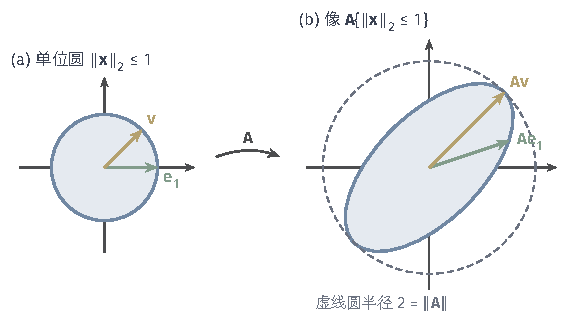
\includegraphics[width=95.1mm]{figures/02-abstract-mathematics/03-function-spaces/tikz/c2-operator-norm-stretch/figure.pdf}
  \caption{算子范数是单位球的像离原点最远的距离。(a)~平面单位圆及两个单位向量$\bm e_1$（绿）、$\bm v=(1,1)^{\top}/\sqrt2$（黄）；(b)~在$\bm A=\bigl[\begin{smallmatrix}3/2&1/2\\1/2&3/2\end{smallmatrix}\bigr]$作用下，单位圆变为旋转$45^\circ$、半轴为$2$与$1$的椭圆。$\bm A\bm e_1$的长度约为$1.58$，$\bm A\bm v$的长度为$2$，恰好触到半径为$\|\bm A\|=2$的虚线圆。}
  \label{fig:lfo-operator-norm-stretch}
\end{figure}

\paragraph{上确界未必取到}
在平面例子中，最大伸长由某个单位向量实际取到；无限维中，式~\eqref{eq:lfo-operator-norm}的上确界不一定是某个输入的输出。在$\ell^2$上令$A(x_1,x_2,x_3,\ldots)=\bigl(\tfrac12x_1,\tfrac23x_2,\tfrac34x_3,\ldots\bigr)$，即第$n$个坐标乘以$n/(n+1)$。每个坐标被乘以小于$1$的因子，故$\|Ax\|<\|x\|$对一切$x\neq0$成立；另一方面，标准单位向量满足$\|Ae_n\|=n/(n+1)\to1$，所以$\|A\|=1$，但没有任何单位向量使$\|Ax\|=1$。因此$\|A\|$应理解为“最小的统一上界”，不能无条件称为“最大输出”。

\paragraph{加权积分的范数}
回到加权积分$Wf=\int_0^1wf\,dt$，输入空间取$C([0,1])$配一致范数$\|f\|_\infty$。由$|Wf|\leq\int_0^1w|f|\,dt\leq\|f\|_\infty\int_0^1w\,dt$得$\|W\|\leq\int_0^1w\,dt$；取$f\equiv1$时等号成立，所以$\|W\|=\int_0^1w\,dt$。例如$w(t)=2t$时$\|W\|=1$。同一个读数规则若改用$L^2$范数衡量输入，算子范数会变成另一个数，第~\ref{sec:lfo-point-evaluation}节将用Hölder不等式计算。

\paragraph{求导：有界性取决于范数}
现在看求导$D$。若输入空间取$C^1([0,2\pi])$，并配上同时控制函数值与导数的范数
\[
 \|u\|_{C^1}=\|u\|_\infty+\|u'\|_\infty ,
\]
则$\|Du\|_\infty=\|u'\|_\infty\leq\|u\|_{C^1}$，$D:C^1([0,2\pi])\to C([0,2\pi])$是有界算子，$\|D\|\leq1$。取$u_n(x)=\sin(nx)/n$，有$\|Du_n\|_\infty=1$而$\|u_n\|_{C^1}=1+1/n$，比值趋于$1$，所以$\|D\|=1$；这个上确界同样不被取到，因为取到它需要$\|u\|_\infty=0$。

若在同一个函数集合$C^1([0,2\pi])$上只用一致范数$\|u\|_\infty$衡量输入，情况就完全不同。取$u_n(x)=\sin(nx)$，则
\[
 \|u_n\|_\infty=1,\qquad \|Du_n\|_\infty=\|n\cos(nx)\|_\infty=n .
\]
输出与输入的范数之比为$n$，可以任意大，所以不存在统一常数。图~\ref{fig:lfo-sine-derivative}显示了原因：振幅不变而频率升高时，函数值始终在$[-1,1]$中，斜率却按频率放大。输入上一个一致范数很小的高频扰动，可以使导数产生很大的误差。

\begin{figure}[!htb]
  \centering
  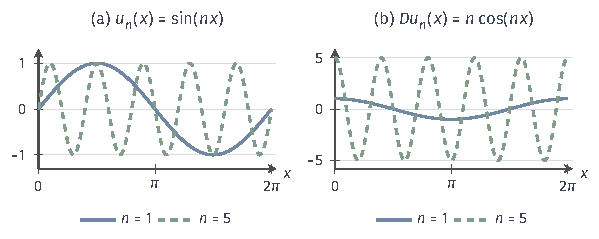
\includegraphics[width=101.5mm]{figures/02-abstract-mathematics/03-function-spaces/tikz/c2-sine-derivative/figure.pdf}
  \caption{求导对高频输入放大误差。(a)~$u_n(x)=\sin(nx)$在$n=1$（蓝实线）与$n=5$（绿虚线）时的一致范数都为$1$；(b)~导数$n\cos(nx)$的一致范数为$n$。若输入只用一致范数衡量，求导不存在统一的误差界；改用同时计入导数的$C^1$范数后，同一作用规则变为有界算子。}
  \label{fig:lfo-sine-derivative}
\end{figure}

这个例子说明，说一个算子是否有界时，必须同时交代三件事：作用规则、定义域以及定义域上的范数。把$D$看成从$C([0,2\pi])$到自身的算子时，它的定义域$D(D)=C^1([0,2\pi])$只是$C([0,2\pi])$的一个子空间，而且它在一致范数下无界，这类算子称为\term{无界算子}（unbounded operator）。对这类算子必须明确写出$D(A)$，不能把它当作已经定义在整个$X$上；第~\ref{sec:lfo-closed-graph}节还会回到求导，说明怎样选择定义域上的范数使它重新成为有界算子。

\subsection{算子的运算与算子空间}
\label{sec:lfo-operator-space}

\paragraph{加法、数乘与复合}
同一对空间之间的两个算子可以相加和数乘：对$A,B:X\to Y$及标量$\alpha$，令$(A+B)x=Ax+Bx$，$(\alpha A)x=\alpha Ax$。若$A:X\to Y$、$B:Y\to Z$，前者的输出空间正是后者的输入空间，就可以复合，$(BA)x=B(Ax)$，先作用$A$、再作用$B$，与矩阵乘积的顺序相同。这些运算都保持线性，问题是它们是否保持有界，以及范数怎样变化。

\begin{theorem}[算子运算的范数估计]
\label{thm:lfo-operator-algebra}
设$A,B:X\to Y$有界，$C:Y\to Z$有界，$\alpha\in\mathbb F$。则$A+B$、$\alpha A$与$CA$都有界，且
\[
 \|A+B\|\leq\|A\|+\|B\|,\qquad \|\alpha A\|=|\alpha|\,\|A\|,\qquad \|CA\|\leq\|C\|\,\|A\| .
\]
\end{theorem}

\begin{proof}
三个估计都先对单个输入成立，再对单位球取上确界。对$\|x\|\leq1$，由$Y$中的三角不等式，$\|(A+B)x\|\leq\|Ax\|+\|Bx\|\leq\|A\|+\|B\|$；数乘的等式直接来自范数的齐次性。复合时先用$C$的界，再用$A$的界：$\|C(Ax)\|\leq\|C\|\,\|Ax\|\leq\|C\|\,\|A\|$。
\end{proof}

复合的估计一般是严格不等式。在平面上取$\bm A=\operatorname{diag}(1,0)$、$\bm C=\operatorname{diag}(0,1)$，两者范数都是$1$，乘积却是零矩阵：$\bm A$保留的方向恰好被$\bm C$消去。每个空间都有自己的单位算子$I_X$和零算子，写复合时须分清它们属于哪个空间，例如$I_YA=A=AI_X$。

\paragraph{先投影再读数}
标量读数可以与一般变换使用同一套运算。在$H=L^2(0,1)$中，令$M$为常数函数组成的一维子空间。常数$1$是$M$中的单位向量，所以投影为$Pf=\langle1,f\rangle\cdot1=\bigl(\int_0^1f\,dt\bigr)\cdot1$。再在$M$上定义读数$\ell(c\cdot1)=c$，即读出这个常数的值。复合$\ell P:H\to\mathbb R$给出$\ell P(f)=\int_0^1f\,dt$，是一个有界线性泛函，$\|\ell P\|\leq\|\ell\|\,\|P\|=1$。

这个例子还说明了复合中定义域的作用。“读出某点的值”对一般的$L^2$等价类没有意义（第~\ref{sec:lfo-point-evaluation}节将说明原因），但$P$的输出已经落在常数函数组成的子空间中，在那里读一个值是有良定义的。复合是否合法，取决于前一个算子的输出是否落在后一个算子的定义域中，而不取决于两个规则单独看起来是否合理。

\paragraph{有界算子组成的空间}
把从$X$到$Y$的全部有界线性算子收集起来，记为$\mathcal B(X,Y)$；$X=Y$时简记$\mathcal B(X)$。由定理~\ref{thm:lfo-operator-algebra}，$\mathcal B(X,Y)$在加法和数乘下封闭，而且算子范数满足范数的三条公理（$\|A\|=0$意味着$Ax=0$对一切$x$成立，即$A=0$），所以$\mathcal B(X,Y)$本身是赋范空间。第~\ref{chap:operator-spectra-equations}章要用有限秩算子逼近一般算子、对算子级数求和，这些操作需要算子列的极限仍然留在$\mathcal B(X,Y)$中。

\begin{theorem}[算子空间的完备性]
\label{thm:lfo-operator-space-complete}
设$X$是赋范空间，$Y$是Banach空间。则$\mathcal B(X,Y)$在算子范数下是Banach空间。
\end{theorem}

证明的思路是先对每个固定输入找到输出的极限，拼成一个候选算子，再验证它线性、有界，最后把逐点收敛加强为算子范数收敛。

\begin{proof}
设$(A_n)$是$\mathcal B(X,Y)$中的Cauchy列。

\emph{第一步：逐点构造极限。}对固定的$x\in X$，$\|A_nx-A_mx\|\leq\|A_n-A_m\|\,\|x\|$，所以$(A_nx)$是$Y$中的Cauchy列。$Y$完备，于是极限存在，记为$Ax=\lim_nA_nx$。

\emph{第二步：极限映射线性且有界。}线性由极限的线性得到：$A(\alpha x+\beta z)=\lim_n(\alpha A_nx+\beta A_nz)=\alpha Ax+\beta Az$。Cauchy列有界，设$\|A_n\|\leq K$，则$\|Ax\|=\lim_n\|A_nx\|\leq K\|x\|$，故$A\in\mathcal B(X,Y)$。

\emph{第三步：算子范数收敛。}任给$\varepsilon>0$，取$N$使$n,m\geq N$时$\|A_n-A_m\|<\varepsilon$。对任意$\|x\|\leq1$及$n\geq N$，$\|A_nx-A_mx\|<\varepsilon$；固定$n$而令$m\to\infty$，得$\|A_nx-Ax\|\leq\varepsilon$。这个界对单位球上一切$x$同时成立，所以$\|A_n-A\|\leq\varepsilon$。
\end{proof}

证明只用到了输出空间$Y$的完备性，输入空间$X$不必完备。取$Y=\mathbb F$，就得到第~\ref{sec:lfo-hahn-banach}节要用的结论：任何赋范空间上的有界线性泛函全体都组成Banach空间。

\paragraph{绝对收敛的算子级数}
完备性的一个直接用途是对算子级数求和。若$A_k\in\mathcal B(X,Y)$且$\sum_k\|A_k\|<\infty$，则部分和$S_n=\sum_{k\leq n}A_k$满足$\|S_n-S_m\|\leq\sum_{k=m+1}^n\|A_k\|$（$n>m$），右端是收敛正项级数的尾部，所以$(S_n)$是Cauchy列，由定理~\ref{thm:lfo-operator-space-complete}收敛到某个$S\in\mathcal B(X,Y)$。第~\ref{sec:ose-neumann}节将用这一点对$\sum_kK^k$求和，解第二类积分方程。

\subsection{算子列的收敛}
\label{sec:lfo-operator-convergence}

上一小节在算子范数下讨论Cauchy列，这只是算子列收敛的一种方式。实际计算中更常见的情形是：用一列逐渐精细的近似算子$A_n$代替$A$，对手中的每个输入，近似输出都会越来越准。这种“对每个输入分别收敛”的要求，与“对全部单位输入同时控制误差”的要求，强弱并不相同。

\begin{definition}[强算子收敛与算子范数收敛]
\label{def:lfo-operator-convergence}
设$A_n,A\in\mathcal B(X,Y)$。若对每个$x\in X$都有$\|A_nx-Ax\|\to0$，则称$A_n$\term{强算子收敛}（strong operator convergence）到$A$；若$\|A_n-A\|\to0$，则称$A_n$\term{算子范数收敛}（convergence in operator norm）到$A$。
\end{definition}

两种收敛的量词次序不同。强算子收敛先固定输入$x$，再让$n$趋于无穷，收敛快慢可以随$x$变化；算子范数收敛要求一个只依赖$n$的误差界$\|A_n-A\|$，对单位球上的全部输入同时有效。由$\|A_nx-Ax\|\leq\|A_n-A\|\,\|x\|$，算子范数收敛蕴含强算子收敛。

强算子收敛描述的是算子列，变化的对象是算子；第~\ref{sec:lfo-weak}节的弱收敛描述的是一列空间元素，两者不能混用。下面的例子说明，强算子收敛不能反过来推出算子范数收敛。

\paragraph{截断投影$P_n\to I$}
设$H$是无限维可分Hilbert空间，$(e_k)_{k\geq1}$是第~\ref{sec:fs-orthonormal-bases}节的标准正交基，$P_n$是到$\operatorname{span}\{e_1,\ldots,e_n\}$的正交投影，$P_nx=\sum_{k\leq n}\langle e_k,x\rangle e_k$。对固定的$x$，第~\ref{sec:fs-orthogonal-expansion}节的Parseval等式给出
\[
 \|x-P_nx\|^2=\sum_{k>n}|\langle e_k,x\rangle|^2\longrightarrow0 ,
\]
因为右端是收敛级数$\sum_k|\langle e_k,x\rangle|^2=\|x\|^2$的尾部。所以$P_n$强算子收敛到单位算子$I$。

另一方面，对每个$n$，被截掉的单位向量$e_{n+1}$满足$P_ne_{n+1}=0$，于是$\|(I-P_n)e_{n+1}\|=1$。又因为$I-P_n$是到正交补的投影，$\|I-P_n\|\leq1$，所以$\|I-P_n\|=1$对一切$n$成立，$P_n$不按算子范数收敛到$I$。

图~\ref{fig:lfo-projection-strong-norm}给出了两个单位向量的截断误差。系数为$2^{-k/2}$的$x$截断误差为$2^{-n/2}$，衰减很快；系数与$1/k$成比例的$y$衰减慢得多，$n=30$时误差仍约为$0.14$。每个固定向量的误差都趋于零，但不同向量的速度可以任意慢，而被截掉的那个基向量的误差始终是$1$。这说明逐个函数可以被有限维子空间逼近，并不意味着同一个有限维子空间能以任意精度统一逼近整个单位球；第~\ref{sec:ose-finite-rank}节将看到，紧算子恰好是能被有限秩算子按算子范数逼近的那一类。

\begin{figure}[!htb]
  \centering
  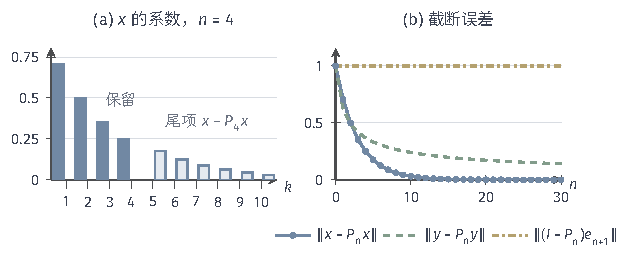
\includegraphics[width=107.2mm]{figures/02-abstract-mathematics/03-function-spaces/tikz/c2-projection-strong-norm/figure.pdf}
  \caption{截断投影的强收敛与算子范数不收敛。(a)~单位向量$x$的系数$c_k=2^{-k/2}$，$P_4$保留深色的前四项，浅色尾项构成误差$x-P_4x$；(b)~截断误差随保留项数$n$的变化：$\|x-P_nx\|=2^{-n/2}$（蓝），系数与$1/k$成比例的单位向量$y$的误差衰减较慢（绿虚线），而对被截掉的基向量$e_{n+1}$，误差始终为$1=\|I-P_n\|$（黄点划线）。}
  \label{fig:lfo-projection-strong-norm}
\end{figure}

\paragraph{有限个输入上的统一控制}
强算子收敛虽然不能控制整个单位球，对有限个输入却可以同时控制：若$x^{(1)},\ldots,x^{(m)}$是固定的输入，对每个$i$取$N_i$使误差小于$\varepsilon$，再取$N=\max_iN_i$即可。在$P_n$的例子中，失去统一控制的原因是单位球中有无穷多个相互正交的方向，每个$P_n$只能照顾其中有限个。第~\ref{sec:lfo-uniform-boundedness}节将证明，在Banach空间上，强算子收敛的算子列至少有统一的范数上界，这是算子列能被逐点控制时还剩下的统一信息。

% 第2章第2节：线性泛函的表示（积分读取与点值读取、Riesz表示、有限观测与坐标表示）。

\section{线性泛函的表示}
\label{sec:lfo-functional-representation}

本节固定标量输出，研究一个读数规则怎样写成积分权重或空间中的一个方向。顺序上先检查读数规则对空间元素是否有良定义、是否连续，再讨论表示；表示公式以这些条件为前提，不能反过来替它们作证。

\subsection{积分读取与点值读取}
\label{sec:lfo-point-evaluation}

\paragraph{加权积分读取}
最常见的读数是加权平均：给定权重$g$，读出$\int fg\,d\mu$。在测度空间$(\Omega,\mathcal F,\mu)$上取$1\leq p\leq\infty$，并设$q$是共轭指数，即$1/p+1/q=1$（$p=1$时$q=\infty$，$p=\infty$时$q=1$）。对$g\in L^q(\mu)$，令
\begin{equation}
 L_g(f)=\int_\Omega fg\,d\mu\qquad(f\in L^p(\mu)).
 \label{eq:lfo-integral-reading}
\end{equation}
第~\ref{sec:fs-holder-minkowski}节的Hölder不等式给出$|L_g(f)|\leq\int|fg|\,d\mu\leq\|f\|_p\|g\|_q$，所以积分是有限的，$L_g$是有界线性泛函，且$\|L_g\|\leq\|g\|_q$。第~\ref{sec:lfo-lp-dual}节将证明，在$\sigma$有限测度与$1\leq p<\infty$的条件下这里其实是等号。

$L_g$作用在等价类上是合理的：若$f=\tilde f$几乎处处成立，则$fg=\tilde fg$几乎处处成立，两者积分相同，所以$L_g$的值不依赖代表的选取。这一点看似平凡，却正是积分读取能够在$L^p$上使用的原因。

举一个可以复算的例子。在$L^2(0,1)$上取$g=\mathbf 1_{[0,1/2]}$，$L_g(f)=\int_0^{1/2}f\,dt$读出前半段的累计。Hölder不等式给出$\|L_g\|\leq\|g\|_2=1/\sqrt2$；取$f=g$，则$L_g(g)=1/2$而$\|g\|_2=1/\sqrt2$，比值正好是$1/\sqrt2$，所以$\|L_g\|=1/\sqrt2$。同一规则在$C([0,1])$的一致范数下的范数是$1/2$（取$f\equiv1$），两个数不同，因为输入误差的衡量方式不同。

\paragraph{连续函数的点值读取}
另一类读数是读出某一点的值。设$K$是紧致度量空间，$x\in K$固定。在$C(K)$上配一致范数，令$\delta_x(f)=f(x)$，称为在$x$处的\term{点值泛函}（point evaluation functional）。由$|f(x)|\leq\sup_K|f|=\|f\|_\infty$，$\delta_x$是有界线性泛函，$\|\delta_x\|\leq1$；取$f\equiv1$得$\|\delta_x\|=1$。

两种读数都输出一个标量，但依靠的空间结构不同：积分读取依靠积分对零测集不敏感，点值读取依靠一致范数对每一点都有控制。把点值读取搬到积分空间中，这两种结构就发生冲突。

\paragraph{等价类上没有点值}
在Lebesgue测度下的$L^p(0,1)$中，单点$\{x_0\}$的测度为零。改变一个函数在$x_0$处的值，得到的函数与原函数几乎处处相等，属于同一个等价类，例如$f$与$f+\mathbf 1_{\{x_0\}}$。同一个等价类在$x_0$处可以有任何值，所以“读出$x_0$处的值”在$L^p$上根本没有良定义，谈不上是否有界。

\paragraph{窄尖峰：连续代表也不够}
或许可以只考虑连续函数，因为连续代表若存在则唯一。但即使把对象限制在$C([0,1])$中、用$L^2$范数衡量误差，点值仍然不受控制。取贴着左端点、宽为$1/n$、高为$1$的尖峰
\[
 \tau_n(t)=\max(1-nt,\,0)\qquad(t\in[0,1]).
\]
它连续，$\delta_0(\tau_n)=\tau_n(0)=1$，而直接积分得
\[
 \|\tau_n\|_2^2=\int_0^{1/n}(1-nt)^2\,dt=\frac{1}{3n}\longrightarrow0 .
\]
图~\ref{fig:lfo-point-spike}画出了$n=4,10,25$三个尖峰：$L^2$范数从约$0.289$降到约$0.115$，左端点的值始终是$1$。所以不存在常数$C$使$|f(0)|\leq C\|f\|_2$对一切连续$f$成立，点值泛函在$(C([0,1]),\|\cdot\|_2)$上无界。

\begin{figure}[!htb]
  \centering
  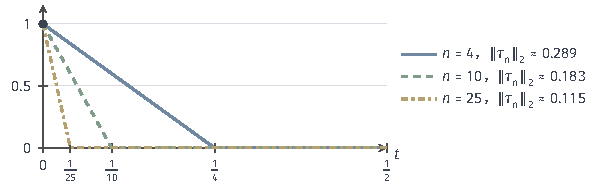
\includegraphics[width=101.7mm]{figures/02-abstract-mathematics/03-function-spaces/tikz/c2-point-spike/figure.pdf}
  \caption{窄尖峰使点值不受$L^2$范数控制。尖峰$\tau_n(t)=\max(1-nt,0)$在$n=4,10,25$时的图像（蓝实线、绿虚线、黄点划线）。左端点的值恒为$1$（黑点），而$\|\tau_n\|_{L^2(0,1)}=1/\sqrt{3n}$随$n$增大趋于零。}
  \label{fig:lfo-point-spike}
\end{figure}

\paragraph{原子测度改变结论}
上面的困难来自单点的测度为零。若测度在$x_0$处有正的质量，结论就会改变。在$[0,1]$上取$\mu=\lambda+\delta_{x_0}$，其中$\lambda$是Lebesgue测度，$\delta_{x_0}$是集中在$x_0$的单位质量。此时$\mu(\{x_0\})=1$，改变$x_0$处的值会改变等价类，于是$f(x_0)$对$L^2(\mu)$的元素有良定义，并且
\[
 |f(x_0)|^2=\int_{\{x_0\}}|f|^2\,d\mu\leq\int|f|^2\,d\mu=\|f\|_{L^2(\mu)}^2 .
\]
正测度的单点原子与零测单点必须区分。一般的积分空间不支持点值读取；第~\ref{chap:rkhs}章将专门研究点值读取连续的Hilbert函数空间，第~\ref{sec:sob-embedding}节则说明控制导数能在什么条件下恢复点值的连续性。

\subsection{Hilbert空间中的Riesz表示}
\label{sec:lfo-riesz}

\paragraph{每个方向给出一个读数}
在Hilbert空间$H$中，任取$h\in H$，令$L_h(f)=\langle h,f\rangle$。按全书的约定，内积对第二个变量线性，所以$L_h$是线性泛函。Cauchy--Schwarz不等式给出$|L_h(f)|\leq\|h\|\,\|f\|$，即$\|L_h\|\leq\|h\|$；$h\neq0$时取$f=h/\|h\|$，得$L_h(f)=\|h\|$，于是$\|L_h\|=\|h\|$。每个方向都是一个读数规则，读数的范数等于方向的长度。

反过来的问题更有用：给定一个有界线性读数$L$，是否一定存在方向$h$，使读数就是与$h$做内积？若是，就可以用空间中的几何（正交、投影、长度）来研究读数。

\paragraph{核与正交方向}
先观察一个非零有界线性泛函$L$的核$N=\ker L=\{f:L(f)=0\}$。它是线性子空间；又因为$L$连续，若$f_n\in N$且$f_n\to f$，则$L(f)=\lim L(f_n)=0$，所以$N$是闭子空间。$N$还“只差一维”：任取$w\notin N$，每个$f$都可以写成
\[
 f=\Bigl(f-\frac{L(f)}{L(w)}w\Bigr)+\frac{L(f)}{L(w)}w ,
\]
括号中的元素在$L$下的值为零，属于$N$。所以$H=N+\operatorname{span}\{w\}$。若进一步把$w$取在$N$的正交补中，读数$L(f)$就只取决于$f$沿$w$方向的分量，这正是表示向量的来源。由此得到的结论称为\term{Riesz表示定理}（Riesz representation theorem）。

\begin{theorem}[Riesz表示定理]
\label{thm:lfo-riesz}
设$H$是Hilbert空间，$L:H\to\mathbb F$是有界线性泛函。则存在唯一的$h_L\in H$，使
\begin{equation}
 L(f)=\langle h_L,f\rangle\qquad(f\in H),
 \label{eq:lfo-riesz}
\end{equation}
并且$\|L\|=\|h_L\|$。
\end{theorem}

证明分三步：用投影找出与核正交的方向，用这个方向写出表示，再验证唯一性与范数等式。

\begin{proof}
$L=0$时取$h_L=0$。下设$L\neq0$，于是闭子空间$N=\ker L$不是全空间。

\emph{第一步：找与核正交的方向。}取$v$使$L(v)\neq0$。由第~\ref{sec:fs-projection}节的正交投影定理，$v=P_Nv+w$，其中$P_Nv\in N$，$w=v-P_Nv\perp N$。由$L(w)=L(v)-L(P_Nv)=L(v)\neq0$知$w\neq0$。

\emph{第二步：写出表示。}对任意$f\in H$，前面已说明$f-\frac{L(f)}{L(w)}w\in N$，它与$w$正交：
\[
 0=\Bigl\langle w,\ f-\frac{L(f)}{L(w)}w\Bigr\rangle=\langle w,f\rangle-\frac{L(f)}{L(w)}\|w\|^2 .
\]
这里用到内积对第二个变量线性。解出$L(f)=\frac{L(w)}{\|w\|^2}\langle w,f\rangle$。令
\begin{equation}
 h_L=\frac{\overline{L(w)}}{\|w\|^2}\,w ,
 \label{eq:lfo-riesz-direction}
\end{equation}
由于内积对第一个变量共轭线性，$\langle h_L,f\rangle=\frac{L(w)}{\|w\|^2}\langle w,f\rangle=L(f)$。

\emph{第三步：唯一性与范数。}若$h,h'$都满足式~\eqref{eq:lfo-riesz}，则$\langle h-h',f\rangle=0$对一切$f$成立，取$f=h-h'$得$h=h'$。范数等式正是本小节开头对$L_h$的计算。
\end{proof}

式~\eqref{eq:lfo-riesz-direction}中的共轭在实空间中消失；在复空间中，它使对应$L\mapsto h_L$是共轭线性的：$h_{\alpha L}=\bar\alpha h_L$。这是内积对第一个变量共轭线性这一约定的直接后果。

\paragraph{读数的几何}
图~\ref{fig:lfo-riesz-kernel}在实平面的二维截面上画出了这个构造。核$N$是一条过原点的直线，表示向量$h_L$与它垂直；读数相等的点组成平行于$N$的直线，读数每增加$\|h_L\|^2$，水平线沿$h_L$方向平移一个$\|h_L\|$的距离。任何$f$都分解为$N$中的分量与沿$h_L$的分量，前者对读数没有贡献，后者的长度决定读数。读数大的方向就是$h_L$本身，这也解释了$\|L\|=\|h_L\|$：在单位球上，沿$h_L$方向的单位向量读到的值最大。

\begin{figure}[!htb]
  \centering
  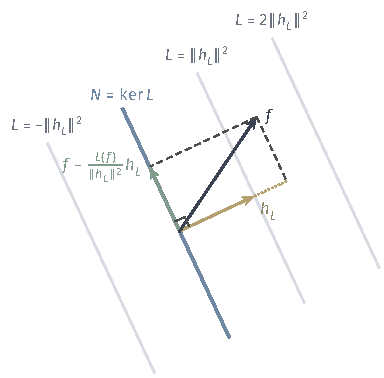
\includegraphics[width=65.1mm]{figures/02-abstract-mathematics/03-function-spaces/tikz/c2-riesz-kernel/figure.pdf}
  \caption{Riesz表示的几何示意（实空间中的二维截面）。核$N=\ker L$（蓝线）是闭子空间，表示向量$h_L$（黄）与之正交；灰线是读数$L=c$的水平集，平行于$N$。元素$f$减去沿$h_L$的分量$\frac{L(f)}{\|h_L\|^2}h_L$后落入$N$（绿），因此读数只由$f$沿$h_L$方向的分量决定。}
  \label{fig:lfo-riesz-kernel}
\end{figure}

\paragraph{$L^2$中的读数与方向}
在$L^2(0,1)$中，几个熟悉的读数对应的方向都可以直接写出。整体平均$L(f)=\int_0^1f\,dt=\langle1,f\rangle$对应常数$h_L=1$，$\|L\|=1$。前半段平均$L(f)=2\int_0^{1/2}f\,dt$对应$h_L=2\cdot\mathbf 1_{[0,1/2]}$，$\|L\|=\|h_L\|_2=2\cdot(1/2)^{1/2}=\sqrt2$。加权读数$L(f)=\int_0^1tf(t)\,dt$对应$h_L(t)=t$，$\|L\|=(\int_0^1t^2\,dt)^{1/2}=1/\sqrt3$。正交展开中的第$k$个系数$f\mapsto\langle e_k,f\rangle$对应$h_L=e_k$。抽象的读数规则由此变成了与一个固定函数的比较，读数的大小就是$f$与这个函数的相关程度。

\paragraph{表示以有界为前提}
Riesz表示定理需要两个前提，缺一不可。第一，$L$必须已经有界。在$C([0,1])$上配$L^2$内积，点值$\delta_0$无界；它也确实没有表示函数：若有连续$h$使$f(0)=\int_0^1hf\,dt$对一切连续$f$成立，代入尖峰$\tau_n$，左端恒为$1$，右端的绝对值不超过$\|h\|_2\|\tau_n\|_2\to0$，矛盾。定理不能替点值读取证明连续性，连续性必须事先单独检验。

第二，空间必须完备。仍在$C([0,1])$上配$L^2$内积，读数$L(f)=\int_0^{1/2}f\,dt$满足$|L(f)|\leq\|f\|_2/\sqrt2$，是有界的。在完备的$L^2(0,1)$中它的表示方向是$\mathbf 1_{[0,1/2]}$，但这个函数没有连续代表，不在$C([0,1])$中。所以在不完备的内积空间里，有界读数可以没有表示向量；证明中用到的正交投影定理依赖完备性，此处失效。

最后，Riesz表示只处理标量输出。输出为向量的观测，例如同时读出两个端点值$(f(0),f(1))$，要逐个分量作为标量泛函处理，各分量分别有自己的表示方向（若它们有界），不能未经说明就当作一个泛函。

\subsection{有限观测与坐标表示}
\label{sec:lfo-finite-observations}

实际中我们只能对函数做有限次读数，并且常把候选函数限制在一个有限维空间里。本小节说明在这种设定下，读数、坐标和函数之间怎样用矩阵联系，以及有限条读数能否唯一确定一个函数。

\paragraph{观测矩阵}
设候选函数属于有限维子空间$V=\operatorname{span}\{\varphi_1,\ldots,\varphi_m\}$，其中$\varphi_1,\ldots,\varphi_m$线性无关，每个$f\in V$唯一地写成$f=\sum_{j=1}^mc_j\varphi_j$，系数向量记为$\bm c=(c_1,\ldots,c_m)^{\top}$。再设$L_1,\ldots,L_n$是$V$上的线性读数。由线性，
\[
 L_i(f)=\sum_{j=1}^mc_jL_i(\varphi_j)\qquad(i=1,\ldots,n).
\]
令$\bm A\in\mathbb F^{n\times m}$，$\bm A_{i,j}=L_i(\varphi_j)$，称为\term{观测矩阵}（observation matrix），则读数向量$\bm r=(L_1(f),\ldots,L_n(f))^{\top}$满足
\begin{equation}
 \bm r=\bm A\bm c .
 \label{eq:lfo-observation-matrix}
\end{equation}
矩阵的第$i$行是第$i$条读数规则在各个基函数上的取值，第$j$列是第$j$个基函数在全部读数下留下的记录。点值读数给出$\bm A_{i,j}=\varphi_j(x_i)$，积分读数给出$\bm A_{i,j}=\int\varphi_jg_i\,d\mu$；代入之前仍须核对每条读数在$V$上有良定义。

\paragraph{仿射函数的两次读数}
取$V$为$[0,1]$上的仿射函数，基为$\varphi_1=1$、$\varphi_2=t$，$f=c_1+c_2t$。读$f(0)$与$f(1)$时，
\[
 \bm A=\begin{bmatrix}1&0\\1&1\end{bmatrix},\qquad
 \begin{bmatrix}f(0)\\f(1)\end{bmatrix}=\bm A\begin{bmatrix}c_1\\c_2\end{bmatrix}.
\]
$\bm A$可逆，由$c_1=f(0)$、$c_2=f(1)-f(0)$恢复系数。若只读$f(0)$，$\bm A=[1\ \ 0]$，第二列为零：斜率方向在记录中完全看不见。若改读$f(0)$与整体平均$\int_0^1f\,dt$，第二行变为$(1,1/2)$，矩阵仍可逆。图~\ref{fig:lfo-observation-matrix}(a)(b)对比了一次与两次点值读数的情形。

\paragraph{非标准正交基下的Gram矩阵}
坐标向量$\bm c$与函数$f$一一对应，但坐标的欧氏长度一般不是函数的范数。在内积空间中，记\term{Gram矩阵}（Gram matrix）$\bm G_{j,k}=\langle\varphi_j,\varphi_k\rangle$，则对$f=\sum_jc_j\varphi_j$、$u=\sum_kd_k\varphi_k$有
\[
 \langle f,u\rangle=\sum_{j,k}\bar c_jd_k\langle\varphi_j,\varphi_k\rangle=\bm c^{\mathsf H}\bm G\bm d ,
\]
其中$\bm c^{\mathsf H}$是共轭转置，实情形即$\bm c^{\top}$。只有基标准正交时$\bm G=\bm I$，函数内积才等于系数内积。

仍以$L^2(0,1)$中的基$1,t$为例，$\bm G=\bigl[\begin{smallmatrix}1&1/2\\1/2&1/3\end{smallmatrix}\bigr]$。函数$f=t-1/2$的系数为$\bm c=(-1/2,1)^{\top}$，于是$\|f\|_2^2=\bm c^{\top}\bm G\bm c=\tfrac14-\tfrac12+\tfrac13=\tfrac1{12}$，与直接积分$\int_0^1(t-1/2)^2\,dt=1/12$一致；而系数的欧氏长度平方是$5/4$，差了十五倍。在坐标中计算误差或正交性时，必须带上$\bm G$。

\paragraph{唯一恢复的条件}
读数能否唯一确定候选空间中的函数，归结为观测矩阵的列是否线性无关。

\begin{theorem}[有限维候选的唯一恢复]
\label{thm:lfo-finite-recovery}
设$V$与$L_1,\ldots,L_n$如上，$\bm A$为观测矩阵。则读数向量唯一确定$V$中的函数，当且仅当$\bm A$满列秩，即$\operatorname{rank}\bm A=m$。特别地，这要求$n\geq m$。
\end{theorem}

\begin{proof}
两个候选$f=\sum c_j\varphi_j$与$u=\sum d_j\varphi_j$给出相同读数，当且仅当$\bm A(\bm c-\bm d)=\bm 0$。所以读数唯一确定函数，当且仅当$\bm A\bm z=\bm 0$只有零解，即$\bm A$的$m$列线性无关；这又等价于秩为$m$，而秩不超过行数$n$。
\end{proof}

结论严格限定在给定的候选空间$V$上。图~\ref{fig:lfo-observation-matrix}(c)把候选扩大到二次多项式：基$1,t,t(t-1)$下，两次点值读数的观测矩阵为$\bigl[\begin{smallmatrix}1&0&0\\1&1&0\end{smallmatrix}\bigr]$，第三列为零，函数$t(t-1)$在$t=0,1$处都等于零，在两次读数中看不见。于是$1+t+s\,t(t-1)$对一切$s$给出相同的记录。

\begin{figure}[!htb]
  \centering
  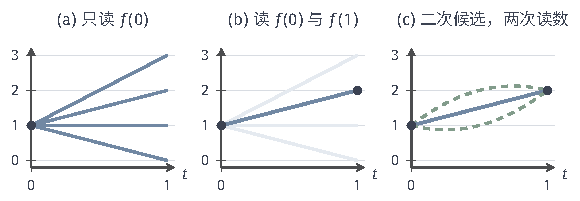
\includegraphics[width=98.2mm]{figures/02-abstract-mathematics/03-function-spaces/tikz/c2-observation-matrix/figure.pdf}
  \caption{有限读数能否确定候选函数。(a)~仿射候选$f=1+bt$（$b=-1,0,1,2$）都满足$f(0)=1$，一次读数无法区分；(b)~再读$f(1)=2$，只剩$b=1$（深蓝线），观测矩阵满列秩；(c)~候选扩大为二次多项式后，$1+t+s\,t(t-1)$（$s=-2,0,2$）在$t=0,1$处的读数完全相同，方向$t(t-1)$不可见。}
  \label{fig:lfo-observation-matrix}
\end{figure}

\paragraph{无限维中有限读数不够}
若候选空间是无限维的，有限条读数永远不能唯一确定函数。线性映射$f\mapsto(L_1(f),\ldots,L_n(f))$从候选空间映到$\mathbb F^n$；它的核若只含零，就会把一个无限维空间单射地放进$n$维空间，这不可能。所以总有非零的$f$使全部读数为零，加到任何候选上都不改变记录。上面的$t(t-1)$只是这种不可见方向在二次多项式中的具体样子。

本小节只建立空间元素、坐标与读数之间的对应。读数带有噪声或彼此不相容时，$\bm r=\bm A\bm c$可能无解，需要另选拟合准则与误差度量；这属于优化问题，可参考\BookChapterRef{chap:optimization}{卷三“优化问题的定义与基本性质”章}。第~\ref{sec:rkhs-finite-observations}节将在点值连续的核空间中，用Riesz表示方向重新组织有限观测。

% 第2章第3节：对偶空间（对偶空间与Hahn--Banach延拓、积分空间的对偶、连续函数空间与测度表示）。

\section{对偶空间}
\label{sec:lfo-dual}

上一节逐个研究读数规则，本节把同一空间上的全部有界线性读数收集成一个空间。我们关心两个问题：这些读数是否多到足以区分任意两个不同的元素，以及在具体的函数空间中，它们究竟长什么样。前一个问题由延拓定理回答，适用于一切赋范空间；后一个问题要按原空间的类型分别回答。

\subsection{对偶空间与泛函延拓}
\label{sec:lfo-hahn-banach}

\begin{definition}[对偶空间]
\label{def:lfo-dual-space}
赋范空间$X$上全部有界线性泛函组成的空间$X^*=\mathcal B(X,\mathbb F)$称为$X$的\term{对偶空间}（dual space），配以泛函范数$\|L\|=\sup_{\|x\|\leq1}|L(x)|$。
\end{definition}

标量域$\mathbb F$是完备的，所以由定理~\ref{thm:lfo-operator-space-complete}，无论$X$本身是否完备，$X^*$总是Banach空间。例如在不完备的多项式空间上配一致范数，它的对偶空间仍然完备。

\paragraph{读数规则与向量表示不是一回事}
对偶空间的元素是读数规则，不是原空间的元素。即使在有限维中，两者的范数也可能不同。在$\mathbb R^2$上配$\ell^1$范数$\|\bm x\|_1=|x_1|+|x_2|$，每个线性泛函都写成$L(\bm x)=a_1x_1+a_2x_2$。由$|L(\bm x)|\leq\max(|a_1|,|a_2|)\,\|\bm x\|_1$，且在$\bm x=\bm e_1$或$\bm e_2$处等号可以成立，得$\|L\|=\max(|a_1|,|a_2|)$。系数向量$\bm a$属于$\mathbb R^2$，但它作为读数的长度要用$\ell^\infty$范数计算，这是\term{对偶范数}（dual norm）的一个例子。

Hilbert空间是特殊情形：Riesz表示定理把每个读数对应到唯一的向量$h_L$，并且$\|L\|=\|h_L\|$，所以$H^*$与$H$可以通过保范数的（复情形下共轭线性的）双射视为同一个空间。对一般空间不能直接写$X^*=X$；第~\ref{sec:lfo-lp-dual}节会看到，$L^p$的对偶在$p\neq2$时由另一个空间$L^q$表示。

\paragraph{读数够不够区分元素}
在Hilbert空间中，若$x\neq0$，读数$\langle x,\cdot\rangle$在$x$处给出$\|x\|^2\neq0$，所以总有连续读数能把$x$与$0$区分开。一般的Banach空间没有内积，无法直接写出这样的读数。我们能做的是先在包含$x$的一维子空间上定义一个读数，再设法把它延拓到全空间，并且不增大它的范数。保证这种延拓存在的是\term{Hahn--Banach定理}（Hahn--Banach theorem）。

\begin{theorem}[Hahn--Banach定理（保范数延拓）]
\label{thm:lfo-hahn-banach}
设$X$是赋范空间，$M\subset X$是线性子空间，$\ell:M\to\mathbb F$是有界线性泛函。则存在$L\in X^*$，使$L|_M=\ell$且$\|L\|=\|\ell\|$。
\end{theorem}

\paragraph{延拓一维：可选范围非空}
以实空间为例看延拓的核心一步。不妨设$\|\ell\|=1$，任取$z\notin M$，要把$\ell$延拓到$M\oplus\operatorname{span}\{z\}$上。线性延拓完全由一个数$t=L(z)$决定：$L(m+sz)=\ell(m)+st$。要求$\|L\|\leq1$，即$|\ell(m)+st|\leq\|m+sz\|$对一切$m\in M$、$s\in\mathbb R$成立。$s=0$时这就是$\|\ell\|\leq1$；$s\neq0$时两边除以$|s|$并把$m/s$重新记为$m$，条件化为
\[
 -\|m+z\|-\ell(m)\leq t\leq\|m+z\|-\ell(m)\qquad(m\in M).
\]
这样的$t$存在，当且仅当左端对$m$的上确界不超过右端对$m'$的下确界，即对一切$m,m'\in M$，
\[
 -\|m+z\|-\ell(m)\leq\|m'+z\|-\ell(m') .
\]
这确实成立，因为$\ell(m')-\ell(m)=\ell(m'-m)\leq\|m'-m\|\leq\|m'+z\|+\|m+z\|$，移项即得。所以可选的$t$组成一个非空区间，任取其中一个就把$\ell$保范数地延拓了一维。

\paragraph{从一维到全空间（补充）}
若$X$可分，取可数稠密集$\{z_1,z_2,\ldots\}$，逐个把$z_k$添进定义域并重复上面的一步，就把$\ell$保范数地延拓到$\operatorname{span}(M\cup\{z_k\})$上；这个子空间稠密，延拓后的泛函一致连续，可以唯一地连续延拓到整个$X$，范数不变。不可分时，“逐个添加”需要用Zorn引理代替归纳法，思路相同。复空间的情形可以先延拓实部$\operatorname{Re}\ell$，再由$L(x)=\operatorname{Re}L(x)-i\operatorname{Re}L(ix)$恢复复线性泛函。这些细节属于补充，主线只需记住条件（$\ell$在子空间上有界）和结论（全空间上存在范数相同的延拓）。

\paragraph{延拓可以不唯一}
图~\ref{fig:lfo-hahn-banach}展示了一维延拓中的那个“非空区间”。在$(\mathbb R^2,\|\cdot\|_1)$中取$M$为横轴，$\ell(s,0)=s$，$\|\ell\|=1$。延拓为$L_t(\bm x)=x_1+tx_2$，由前面对偶范数的计算，$\|L_t\|=\max(1,|t|)$，所以$|t|\leq1$的每个$t$都给出保范数延拓。几何上，水平线$\{L_t=1\}$都经过点$(1,0)$并支撑菱形单位球；菱形在这个顶点处有许多支撑线，延拓因而不唯一。在欧氏范数下，单位圆在$(1,0)$只有一条切线$x_1=1$，延拓唯一。一般地，Hilbert空间中的保范数延拓是唯一的，就是$L=\ell\circ P_{\overline M}$（$\ell$先连续延拓到闭包$\overline M$上）。

\begin{figure}[!htb]
  \centering
  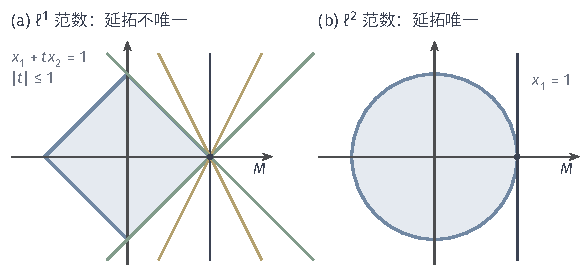
\includegraphics[width=98.9mm]{figures/02-abstract-mathematics/03-function-spaces/tikz/c2-hahn-banach/figure.pdf}
  \caption{保范数延拓与单位球的支撑线。(a)~$(\mathbb R^2,\|\cdot\|_1)$的单位球是菱形，子空间$M$为横轴，$\ell(s,0)=s$。延拓$L_t(\bm x)=x_1+tx_2$在$|t|\leq1$时范数都为$1$，对应的水平线$x_1+tx_2=1$（图中$t=0,\pm\frac12,\pm1$）都过$(1,0)$并支撑菱形；(b)~欧氏单位圆在$(1,0)$只有一条支撑线$x_1=1$，保范数延拓唯一。}
  \label{fig:lfo-hahn-banach}
\end{figure}

\paragraph{读数足以区分元素}
把定理用于一维子空间，就得到本小节开头的问题的答案。

\begin{theorem}[范数的对偶刻画]
\label{thm:lfo-norming-functional}
设$X$是赋范空间，$x\in X$且$x\neq0$。则存在$L\in X^*$，使$\|L\|=1$且$L(x)=\|x\|$。因此对一切$x\in X$，
\begin{equation}
 \|x\|=\sup_{\|L\|\leq1}|L(x)|=\max_{\|L\|\leq1}|L(x)| ,
 \label{eq:lfo-norm-dual}
\end{equation}
并且若$L(x)=L(z)$对一切$L\in X^*$成立，则$x=z$。
\end{theorem}

\begin{proof}
在$M=\operatorname{span}\{x\}$上令$\ell(\alpha x)=\alpha\|x\|$，则$|\ell(\alpha x)|=\|\alpha x\|$，$\|\ell\|=1$。由定理~\ref{thm:lfo-hahn-banach}延拓得到所需的$L$。对一切$\|L'\|\leq1$有$|L'(x)|\leq\|x\|$，而上面的$L$取到等号，故式~\eqref{eq:lfo-norm-dual}成立（$x=0$时两边为零）。最后，若$x\neq z$，对$x-z$取这样的$L$，得$L(x)-L(z)=\|x-z\|\neq0$。
\end{proof}

式~\eqref{eq:lfo-norm-dual}说，一个元素的长度可以由单位读数的最大读值完全恢复。在具体空间中，取到最大值的读数常常可以直接写出。例如在$C([0,1])$中，设$|f|$在$t_0$处取到最大值，则$L=\operatorname{sgn}(f(t_0))\,\delta_{t_0}$就满足$\|L\|=1$、$L(f)=\|f\|_\infty$。定理的价值在于，即使写不出这样的读数，它也保证存在。

凸集的分离、优化问题的对偶以及最优性条件，都是同一延拓思想的几何形式，属于优化问题，可参考\BookChapterRef{chap:constrained-optimization}{卷三“有约束优化的求解”章}。

\subsection{积分空间的对偶}
\label{sec:lfo-lp-dual}

第~\ref{sec:lfo-point-evaluation}节用Hölder不等式说明，每个$g\in L^q$都给出$L^p$上的有界读数$L_g$。本小节回答反方向的问题：$L^p$上的每个有界读数是否都来自某个权重$g$，权重的范数又是否等于读数的范数。为避免共轭记号，先在实值函数上讨论，复情形在小节末交代。

\begin{theorem}[$L^p$的对偶]
\label{thm:lfo-lp-dual}
设$(\Omega,\mathcal F,\mu)$是$\sigma$有限测度空间，$1\leq p<\infty$，$q$为共轭指数。则映射$g\mapsto L_g$，$L_g(f)=\int_\Omega fg\,d\mu$，是从$L^q(\mu)$到$(L^p(\mu))^*$的保范数线性双射，即每个$L\in(L^p)^*$都唯一地写成$L=L_g$，且$\|L\|=\|g\|_q$。
\end{theorem}

证明分两部分：正向说明$\|L_g\|$恰好等于$\|g\|_q$，反向说明每个读数都有这样的权重。

\paragraph{正向：等号由哪个输入取到}
Hölder不等式已给出$\|L_g\|\leq\|g\|_q$，只需找输入取到或逼近等号。设$1<p<\infty$，$g\neq0$。令$f=|g|^{q-1}\operatorname{sgn}(g)$，则$fg=|g|^q$，并且$|f|^p=|g|^{(q-1)p}=|g|^q$（因为$(q-1)p=q$）。于是
\[
 \begin{aligned}
 &L_g(f)=\int|g|^q\,d\mu=\|g\|_q^q,\qquad \|f\|_p=\|g\|_q^{q/p},\\
 &\frac{L_g(f)}{\|f\|_p}=\|g\|_q^{\,q-q/p}=\|g\|_q .
 \end{aligned}
\]
$p=1$、$q=\infty$时等号未必取到，改用逼近：对$\varepsilon>0$，集合$E=\{|g|>\|g\|_\infty-\varepsilon\}$测度为正；由$\sigma$有限，可取$E$中测度有限且为正的部分$E'$，令$f=\operatorname{sgn}(g)\mathbf 1_{E'}/\mu(E')$，则$\|f\|_1=1$而$L_g(f)\geq\|g\|_\infty-\varepsilon$。正向保范数说明映射$g\mapsto L_g$单射。

\paragraph{反向：由读数生成测度}
先设$\mu$有限。给定$L\in(L^p)^*$，对可测集$E$令$\nu(E)=L(\mathbf 1_E)$。证明$\nu$是有限符号测度并对$\mu$绝对连续，就可以调用Radon--Nikodym定理。

有限可加性来自$L$的线性：不交时$\mathbf 1_{E\cup F}=\mathbf 1_E+\mathbf 1_F$。可数可加性来自$L$的连续性，这里用到$p<\infty$：若$E=\bigcup_kE_k$为不交并，则
\[
 \Bigl\|\mathbf 1_E-\sum_{k\leq n}\mathbf 1_{E_k}\Bigr\|_p=\mu\Bigl(\bigcup_{k>n}E_k\Bigr)^{1/p}\longrightarrow0 ,
\]
所以$\sum_{k\leq n}\nu(E_k)\to\nu(E)$。绝对连续性同样直接：$\mu(E)=0$时$\mathbf 1_E$是$L^p$中的零元，$\nu(E)=L(0)=0$。由第~\ref{sec:measure-signed-total-variation}节的Jordan分解（定理~\ref{thm:measure-hahn-jordan}），$\nu$是两个有限测度之差，二者都对$\mu$绝对连续；分别应用Radon--Nikodym定理（定理~\ref{thm:measure-radon-nikodym}），得到可积函数$g$使
\[
 L(\mathbf 1_E)=\int_Eg\,d\mu\qquad(E\in\mathcal F).
\]

\paragraph{反向：从示性函数推广到全空间}
由线性，$L(f)=\int fg\,d\mu$对简单函数$f$成立。接下来说明$g\in L^q$，并把等式推广到全部$L^p$。对$1<p<\infty$，令$E_n=\{|g|\leq n\}$，$f_n=|g|^{q-1}\operatorname{sgn}(g)\mathbf 1_{E_n}$。$f_n$是有界可测函数，可由简单函数一致逼近；在有限测度下一致收敛蕴含$L^p$收敛，两端都随之收敛，所以等式对$f_n$也成立。于是
\[
 \int_{E_n}|g|^q\,d\mu=L(f_n)\leq\|L\|\,\|f_n\|_p=\|L\|\Bigl(\int_{E_n}|g|^q\,d\mu\Bigr)^{1/p},
\]
整理得$(\int_{E_n}|g|^q)^{1/q}\leq\|L\|$。令$n\to\infty$，由单调收敛定理，$\|g\|_q\leq\|L\|$。$p=1$时可类似地在$\{|g|>\|L\|\}$上取示性函数说明该集合零测。既然$g\in L^q$，$L$与$L_g$都是$L^p$上的连续泛函，又在简单函数上相等；第~\ref{sec:fs-density-separability}节说明简单函数在$L^p$中稠密，所以$L=L_g$。

\paragraph{$\sigma$有限情形（补充）}
一般的$\sigma$有限测度把$\Omega$分成可数个测度有限的不交片$\Omega_k$。在每一片上得到$g_k$，由唯一性它们彼此相容，拼成$g=\sum_kg_k\mathbf 1_{\Omega_k}$；对每个有限并的范数估计都不超过$\|L\|$，再用单调收敛得$\|g\|_q\leq\|L\|$。$p=1$时$\sigma$有限不能去掉，$1<p<\infty$时则可以用更细的论证去掉这一假设，这里不展开。

\paragraph{复值函数的配对}
复值情形下，为与内积约定一致，把配对写成$L_g(f)=\int\bar gf\,d\mu$，即对权重取共轭、对输入线性。$p=2$时它正是$\langle g,f\rangle$，定理~\ref{thm:lfo-lp-dual}回到Riesz表示定理。正向构造中的$\operatorname{sgn}(g)$相应换为$g/|g|$（$g=0$处取零）。

\paragraph{一个可复算的范数}
在$L^3(0,1)$上取读数$L(f)=\int_0^1tf(t)\,dt$。共轭指数$q=3/2$，由定理~\ref{thm:lfo-lp-dual}，
\[
 \|L\|=\|t\|_{3/2}=\Bigl(\int_0^1t^{3/2}\,dt\Bigr)^{2/3}=\Bigl(\frac25\Bigr)^{2/3}\approx0.543 ,
\]
取到范数的输入是$f(t)=t^{q-1}=t^{1/2}$。同一个权重在$L^2$中的读数范数是$\|t\|_2=1/\sqrt3\approx0.577$，在$L^1$中是$\|t\|_\infty=1$：指数$p$越小，$L^p$范数对集中在小区域上的输入越宽容，读数相对于它的放大就可能越大。

\paragraph{端点：$L^\infty$的对偶更大}
定理排除了$p=\infty$，这不是技术上的疏漏。$L^1$的对偶是$L^\infty$，但$L^\infty$的对偶一般不能全部由$L^1$表示。以计数测度下的$\ell^\infty$为例。在收敛数列组成的子空间$c$上定义$\ell(x)=\lim_nx_n$，它的范数为$1$。由Hahn--Banach定理，它延拓为某个$L\in(\ell^\infty)^*$。若$L$由某个$g\in\ell^1$表示，即$L(x)=\sum_kg_kx_k$，则由标准单位向量满足$L(e_k)=\lim_n(e_k)_n=0$得每个$g_k=0$，于是$L=0$；可是$L$在常数列$(1,1,\ldots)$上的值为$1$，矛盾。所以$(\ell^\infty)^*$严格大于$\ell^1$；对Lebesgue测度下的$L^\infty(0,1)$也有类似的构造。

这一端点限制为第~\ref{sec:lfo-reflexive}节的反射性和第~\ref{sec:lfo-weak-star}节的弱星收敛保留了准确的入口。有限维和$L^2$中“对偶就是自身”的直觉，不能直接推广到所有积分空间。

\subsection{连续函数空间与测度表示（补充）}
\label{sec:lfo-ck-dual}

本小节转到另一类空间$C(K)$，其中$K$是紧致度量空间，配一致范数，只考虑实值函数。它的读数不再总能写成权重函数的积分，而要用测度表示，相应的结论称为\term{Riesz--Markov--Kakutani表示定理}（Riesz--Markov--Kakutani representation theorem）。

\paragraph{几种读数都是对测度积分}
先看$C([0,1])$上的几个读数：点值$f(0)$，平均$\int_0^1f\,dt$，两者之和，以及端点差$f(1)-f(0)$。它们分别是对测度$\delta_0$、Lebesgue测度$\lambda$、$\delta_0+\lambda$和$\delta_1-\delta_0$的积分，其中$\delta_x$是集中在$x$处的单位质量，称为\term{Dirac测度}（Dirac measure）。一般地，对有限符号Borel测度$\mu$，读数$f\mapsto\int_Kf\,d\mu$满足
\[
 \Bigl|\int_Kf\,d\mu\Bigr|\leq\int_K|f|\,d|\mu|\leq\|f\|_\infty\,|\mu|(K),
\]
其中$|\mu|$是第~\ref{sec:measure-signed-total-variation}节的全变差测度。以端点差为例，$|\mu|(K)=2$，取$f(t)=2t-1$得读数$2$而$\|f\|_\infty=1$，所以读数范数恰为$2$。

\begin{theorem}[$C(K)$的对偶（Riesz--Markov--Kakutani）]
\label{thm:lfo-ck-dual}
设$K$是紧致度量空间。对每个$L\in C(K)^*$，存在唯一的有限符号正则Borel测度$\mu$，使$L(f)=\int_Kf\,d\mu$对一切$f\in C(K)$成立，并且$\|L\|=|\mu|(K)$。
\end{theorem}

\paragraph{证明思路（补充）}
先处理正读数，即$f\geq0$时$L(f)\geq0$的读数。对开集$U$，用$L$在$0\leq f\leq1$且支撑在$U$内的连续函数上的上确界定义$\mu(U)$，再由开集向一般Borel集延拓；正性保证得到的是正测度，连续函数可以从内部逼近开集的示性函数，这保证了$\int f\,d\mu=L(f)$。一般读数分解为两个正读数之差：对$f\geq0$令$L^+(f)=\sup\{L(u):0\leq u\leq f\}$，再线性延拓，则$L^-=L^+-L$也是正读数，两者分别对应测度$\mu^+$、$\mu^-$。在紧致度量空间中，有限Borel测度自动是正则的，正则性保证了表示的唯一性。完整证明见泛函分析教材，主线只使用定理的结论。

\paragraph{测度不必有密度}
表示$C(K)$上读数的是测度，而不是权重函数。点值$\delta_x$对Lebesgue测度没有密度：第~\ref{sec:measure-same-space-comparison}节已经说明，单点质量不能写成“在一点处取无穷大的密度函数”。所以不能把定理~\ref{thm:lfo-ck-dual}理解为“每个读数都有逐点权重”，权重函数只在测度对参考测度绝对连续时才存在。

\paragraph{同一个读数，三种表示}
“读出一点的值”在三种空间中得到三种不同的待遇。在$C(K)$中，它是Dirac测度$\delta_x$，是对偶空间中范数为$1$的元素；在$L^2$中，它根本没有良定义；在第~\ref{chap:rkhs}章的再生核Hilbert空间中，它是有界读数，由Riesz表示对应到一个函数方向$K_x$。表示的形式取决于空间的结构，而不取决于读数规则的文字描述。

\paragraph{与测度弱收敛的关系}
定理~\ref{thm:lfo-ck-dual}把$C(K)^*$与$K$上的有限符号测度等同起来。第~\ref{sec:measure-sequence-convergence}节的概率测度弱收敛要求$\int f\,d\mu_n\to\int f\,d\mu$对一切有界连续$f$成立；在紧致的$K$上，这正是第~\ref{sec:lfo-weak-star}节将要定义的$C(K)^*$中的弱星收敛。测度的弱收敛已有独立的定义和基础，不需要先掌握这里的一般表示定理；本小节只是指出两者在紧致空间上的对应。概率分布之间更细致的比较属于后续问题，可参考\BookChapterRef{chap:information-theory-and-statistical-geometry}{卷四“概率分布的分析与优化”章}。

% 第2章第4节：弱收敛与弱极限（定义与判别、一致有界原理、范数控制、Hilbert空间的弱子列、反射空间、弱星紧性）。

\section{弱收敛与弱极限}
\label{sec:lfo-weak}

本节改用全部连续线性读数来观察一列空间元素：不要求整体误差趋于零，只要求每一个固定的读数都收敛。我们先说明这种收敛比范数收敛少控制了什么，再研究它仍然能控制什么，最后讨论何时能从有界序列中抽出这样收敛的子列。Hilbert空间是主线；一般的反射空间与对偶空间上的弱星收敛作为两个方向的扩展。

\subsection{弱收敛的定义与判别}
\label{sec:lfo-weak-convergence}

\paragraph{单位向量列的两种看法}
在$\ell^2$中考察标准单位向量$e_n$，它的第$n$个坐标为$1$，其余为$0$。任意两个不同的$e_n,e_m$之间距离为$\sqrt2$，所以这一列在范数下不是Cauchy列，没有任何子列范数收敛。可是若只看一个固定的读数$y\in\ell^2$，读数$\langle y,e_n\rangle=\bar y_n$就是$y$的第$n$个坐标；由于$\sum_n|y_n|^2<\infty$，它趋于零。每个固定读数都看到这一列“趋于零”，而整体误差$\|e_n-0\|=1$始终不变。

\begin{definition}[弱收敛]
\label{def:lfo-weak-convergence}
设$X$是赋范空间，$x_n,x\in X$。若对每个$L\in X^*$都有$L(x_n)\to L(x)$，则称$x_n$\term{弱收敛}（weak convergence）到$x$，记为$x_n\rightharpoonup x$，$x$称为弱极限。为区别起见，范数收敛$\|x_n-x\|\to0$也称为强收敛。
\end{definition}

量词的次序是：先固定读数$L$，再令$n\to\infty$。不同读数的收敛速度可以完全不同，定义不要求任何统一的速度。弱极限若存在则唯一：若$x_n\rightharpoonup x$且$x_n\rightharpoonup z$，则$L(x)=L(z)$对一切$L$成立，由定理~\ref{thm:lfo-norming-functional}得$x=z$。这里用到了连续读数足以区分元素。

\paragraph{Hilbert空间中的判别}
在Hilbert空间中，由Riesz表示定理，每个读数都是与某个$y$的内积，所以
\[
 x_n\rightharpoonup x\quad\Longleftrightarrow\quad\langle y,x_n\rangle\to\langle y,x\rangle\ \text{对每个}y\in H .
\]
弱收敛就是与每个固定方向的内积收敛，也就是在每个固定方向上的投影长度收敛。

\begin{theorem}[强收敛蕴含弱收敛]
\label{thm:lfo-strong-implies-weak}
若$\|x_n-x\|\to0$，则$x_n\rightharpoonup x$。
\end{theorem}

\begin{proof}
对每个$L\in X^*$，$|L(x_n)-L(x)|\leq\|L\|\,\|x_n-x\|\to0$。
\end{proof}

反向不成立，$e_n$就是反例：$e_n\rightharpoonup0$，但$\|e_n\|=1$。更一般地，Hilbert空间中任何标准正交序列$(u_n)$都弱收敛到零，因为由Bessel不等式$\sum_n|\langle y,u_n\rangle|^2\leq\|y\|^2$，级数的通项趋于零。

图~\ref{fig:lfo-weak-unit-vectors}以$y_k=1/k$为固定读数：(a)中$e_6$只在第$6$个位置与$y$重叠，读数为$1/6$；(b)中读数$\langle y,e_n\rangle=1/n$逐渐趋于零，而$\|e_n\|$始终为$1$。弱收敛失去的是对整体能量的控制：每个固定方向上的分量都在消失，能量却移到越来越远的坐标上去了。读数的速度也取决于$y$：对单位读数取上确界，$\sup_{\|y\|\leq1}|\langle y,e_n\rangle|=1$，所以不存在对全部单位读数统一的收敛速度，否则就是范数收敛了。

\begin{figure}[!htb]
  \centering
  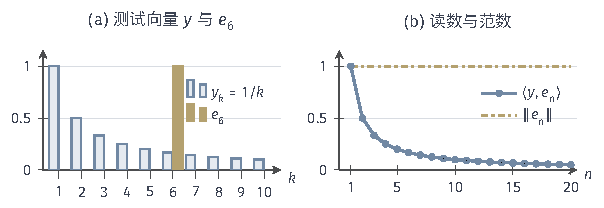
\includegraphics[width=102.3mm]{figures/02-abstract-mathematics/03-function-spaces/tikz/c2-weak-unit-vectors/figure.pdf}
  \caption{$\ell^2$中标准单位向量的弱收敛。(a)~固定读数$y_k=1/k$（浅蓝柱）与$e_6$（黄柱）只在第$6$个坐标重叠；(b)~读数$\langle y,e_n\rangle=1/n$（蓝）趋于零，而范数$\|e_n\|=1$（黄点划线）保持不变。每个固定读数都看到序列趋于零，整体误差却不减小。}
  \label{fig:lfo-weak-unit-vectors}
\end{figure}

\paragraph{振荡的函数}
函数空间中最典型的弱收敛来自振荡。在$L^2(0,2\pi)$中，$\sin(nx)/\sqrt\pi$是标准正交序列，所以$\sin(nx)\rightharpoonup0$。具体地取读数$g=\mathbf 1_{[0,1]}$，得$\int_0^1\sin(nx)\,dx=(1-\cos n)/n\to0$，而$\|\sin(nx)\|_2=\sqrt\pi$保持不变。函数在正负之间越来越快地摆动，任何固定的权重与它相乘再积分时，正负部分都相互抵消。

\paragraph{与测度弱收敛的区别}
第~\ref{sec:measure-sequence-convergence}节也有一个“弱收敛”，但对象和测试都不同。那里变化的是测度$\mu_n$，测试对象是有界连续函数，要求$\int f\,d\mu_n\to\int f\,d\mu$；这里变化的是一个固定线性空间中的元素，测试对象来自该空间的对偶。例如$\delta_{1/n}$作为测度弱收敛到$\delta_0$，但若把它们看成$C([0,1])^*$中的元素，它们之间的全变差距离始终为$2$，在对偶范数下并不收敛；两者的关系要通过第~\ref{sec:lfo-weak-star}节的弱星收敛来说明。两个定义同名，不能只凭名字互换。

\subsection{逐点有界与一致有界}
\label{sec:lfo-uniform-boundedness}

弱收敛只给出逐个读数的信息。我们自然要问：从“每个固定输入上都受控”能否推出某种统一的控制？本小节在Banach空间上给出肯定回答，下一小节再把它用于弱收敛列。

\paragraph{量词能否交换}
设$\{A_\alpha\}_{\alpha\in I}$是$\mathcal B(X,Y)$中的一族算子，并且对每个固定的$x$，$\sup_\alpha\|A_\alpha x\|<\infty$，称为逐点有界。问题是能否推出$\sup_\alpha\|A_\alpha\|<\infty$，即一致有界。前者是“对每个$x$，存在常数$C_x$”，后者是“存在常数$C$，对每个单位$x$”，两者的量词次序不同。

不完备的空间中，答案是否定的。在只有有限项非零的数列组成的空间$c_{00}$上配一致范数，令$L_n(x)=nx_n$。对固定的$x$，$n$超过最后一个非零坐标后$L_n(x)=0$，所以$\sup_n|L_n(x)|<\infty$；可是$\|L_n\|=n$，没有统一上界。下面会看到，完备性正是把逐点有界转为一致有界的关键。

\paragraph{Baire定理}
需要的工具是完备度量空间的一个性质：它不能写成可数个“很瘦”的闭集之并。这一性质称为\term{Baire纲定理}（Baire category theorem）。

\begin{theorem}[Baire纲定理]
\label{thm:lfo-baire}
设$(X,d)$是非空完备度量空间，$F_1,F_2,\ldots$是闭集且$X=\bigcup_kF_k$。则至少有一个$F_k$包含某个开球。
\end{theorem}

\begin{proof}
设每个$F_k$都不含开球，下面构造一个不属于任何$F_k$的点。$F_1$不含开球，所以$X\setminus F_1$是非空开集，可以取闭球$\overline B(x_1,r_1)\subset X\setminus F_1$，$r_1<1$。$F_2$不含开球，所以开球$B(x_1,r_1)$中有点不在$F_2$中，又因$F_2$闭，可取$\overline B(x_2,r_2)\subset B(x_1,r_1)\setminus F_2$，$r_2<1/2$。如此继续，得到嵌套闭球$\overline B(x_k,r_k)$，$r_k<1/k$，且第$k$个球与$F_k$不交。

球心满足$d(x_k,x_m)<r_k$（$m>k$），所以$(x_k)$是Cauchy列。由完备性，$x_k\to x$；每个闭球包含此后的全部球心，故$x\in\overline B(x_k,r_k)$对一切$k$成立，从而$x\notin F_k$对一切$k$成立，与$X=\bigcup_kF_k$矛盾。
\end{proof}

完备性在证明中只用了一次，即保证嵌套球心的极限存在。在$c_{00}$中，同样的嵌套构造可以逼近一个有无穷多非零项的数列，这个极限不在空间中，论证因此失效。下面的\term{一致有界原理}（uniform boundedness principle）把Baire定理用于算子族。

\begin{theorem}[一致有界原理]
\label{thm:lfo-uniform-boundedness}
设$X$是Banach空间，$Y$是赋范空间，$\{A_\alpha\}_{\alpha\in I}\subset\mathcal B(X,Y)$逐点有界，即对每个$x\in X$有$\sup_\alpha\|A_\alpha x\|<\infty$。则$\sup_\alpha\|A_\alpha\|<\infty$。
\end{theorem}

证明按“闭集覆盖—Baire定理给出内点—平移—缩放”的顺序展开。

\begin{proof}
\emph{第一步：层级闭集覆盖空间。}令$F_k=\{x\in X:\sup_\alpha\|A_\alpha x\|\leq k\}$。每个集合$\{x:\|A_\alpha x\|\leq k\}$由连续函数$x\mapsto\|A_\alpha x\|$定义，是闭集，$F_k$是它们的交，也是闭集。逐点有界说明每个$x$属于某个$F_k$，所以$X=\bigcup_kF_k$。

\emph{第二步：某一层含有开球。}$X$完备，由Baire定理，存在$k_0$和开球$B(x_0,r)\subset F_{k_0}$。

\emph{第三步：平移到原点。}对任意$\|z\|<r$，$x_0+z$与$x_0$都在$F_{k_0}$中，于是对每个$\alpha$，
\[
 \|A_\alpha z\|=\|A_\alpha(x_0+z)-A_\alpha x_0\|\leq k_0+k_0=2k_0 .
\]

\emph{第四步：缩放得到统一界。}对任意单位向量$x$及$0<s<r$，$\|sx\|<r$，由上一步$\|A_\alpha x\|=s^{-1}\|A_\alpha(sx)\|\leq2k_0/s$。令$s\to r$，得$\|A_\alpha\|\leq2k_0/r$对一切$\alpha$成立。
\end{proof}

图~\ref{fig:lfo-baire-layers}示意了这个论证。层级集$F_k=kF_1$是对称的闭凸集，一层套一层地覆盖整个空间；Baire定理保证某一层$F_{k_0}$中有一个小球。把这个球平移到原点，两点之差的估计使所有算子在原点附近的小球上一致受控，再用线性缩放推到整个单位球。

\begin{figure}[!htb]
  \centering
  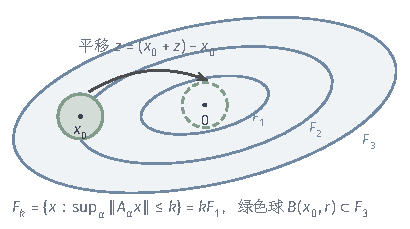
\includegraphics[width=69.3mm]{figures/02-abstract-mathematics/03-function-spaces/tikz/c2-baire-layers/figure.pdf}
  \caption{一致有界原理证明的示意。层级集$F_k=\{x:\sup_\alpha\|A_\alpha x\|\leq k\}$（蓝色嵌套区域）闭、对称且$F_k=kF_1$，它们的并是全空间。Baire定理给出某层（此处$F_3$）中的开球$B(x_0,r)$（绿）；平移到原点后，$z=(x_0+z)-x_0$使$\|z\|<r$时$\|A_\alpha z\|\leq2k_0$，缩放即得$\|A_\alpha\|\leq2k_0/r$。形状只是示意。}
  \label{fig:lfo-baire-layers}
\end{figure}

\paragraph{强收敛的算子列有统一界}
一致有界原理的第一个推论回答了第~\ref{sec:lfo-operator-convergence}节末尾的问题。

\begin{theorem}[Banach--Steinhaus]
\label{thm:lfo-banach-steinhaus}
设$X$是Banach空间，$Y$是赋范空间，$A_n\in\mathcal B(X,Y)$，并且对每个$x$，极限$Ax=\lim_nA_nx$存在。则$\sup_n\|A_n\|<\infty$，$A$是有界线性算子，且$\|A\|\leq\liminf_n\|A_n\|$。
\end{theorem}

\begin{proof}
收敛序列有界，所以$\{A_n\}$逐点有界，由定理~\ref{thm:lfo-uniform-boundedness}一致有界。$A$的线性由极限的线性得到。对单位向量$x$，$\|Ax\|=\lim_n\|A_nx\|\leq\liminf_n\|A_n\|$，对$x$取上确界即得。
\end{proof}

在截断投影的例子中，$\|P_n\|=1$，强极限$I$的范数也是$1$。这个推论说明，Banach空间上的强算子极限不会失去有界性，但它不能改进为算子范数收敛。

\paragraph{同一基础的后续用途}
完备性使量词交换成立，这个基础还会在第~\ref{sec:lfo-open-mapping}节的开映射定理中再用一次，届时直接调用Baire定理，不再重复建立。

\subsection{弱收敛列的范数控制}
\label{sec:lfo-weak-norm}

现在把一致有界原理用于弱收敛列。弱收敛只控制逐个读数，但我们将看到它仍然控制了两件事：序列的范数有统一上界，极限的范数不超过序列范数的下极限。

\begin{theorem}[弱收敛列有界且范数下半连续]
\label{thm:lfo-weak-bounded}
设$X$是赋范空间，$x_n\rightharpoonup x$。则$\sup_n\|x_n\|<\infty$，并且
\begin{equation}
 \|x\|\leq\liminf_{n\to\infty}\|x_n\| .
 \label{eq:lfo-weak-lsc}
\end{equation}
\end{theorem}

\begin{proof}
\emph{有界性。}把每个$x_n$看成对偶空间上的读数：$J_n(L)=L(x_n)$，$L\in X^*$。$J_n$是$X^*$上的线性泛函，它的范数是单位读数在$x_n$上的最大读值，由定理~\ref{thm:lfo-norming-functional}恰好等于$\|x_n\|$。对每个固定的$L$，$J_n(L)=L(x_n)$收敛，因而有界，所以$\{J_n\}$在$X^*$上逐点有界。$X^*$总是Banach空间，由定理~\ref{thm:lfo-uniform-boundedness}得$\sup_n\|x_n\|=\sup_n\|J_n\|<\infty$。

\emph{下半连续。}任取$\|L\|\leq1$，则$|L(x)|=\lim_n|L(x_n)|\leq\liminf_n\|x_n\|$。对$L$取上确界，由式~\eqref{eq:lfo-norm-dual}得式~\eqref{eq:lfo-weak-lsc}。
\end{proof}

证明中用到的完备空间是$X^*$而不是$X$，所以这个结论对不完备的$X$也成立。

\paragraph{不弱收敛的放大序列}
定理给出了一个检验：无界的序列不可能弱收敛。在$\ell^2$中，$\sqrt n\,e_n$的范数趋于无穷，所以它不弱收敛。可以直接找到证据：取$y_k=k^{-3/4}$，$\sum_kk^{-3/2}<\infty$，$y\in\ell^2$，而$\langle y,\sqrt n\,e_n\rangle=n^{1/4}\to\infty$。

\paragraph{范数可以在极限中下降}
式~\eqref{eq:lfo-weak-lsc}可以是严格不等式：$e_n\rightharpoonup0$，$\|0\|=0<1=\liminf\|e_n\|$。弱收敛允许一部分“能量”在极限中消失，例如振荡的$\sin(nx)$弱收敛到零而范数保持$\sqrt\pi$。

\paragraph{Hilbert空间：弱收敛加范数收敛得强收敛}
如果范数没有下降，在Hilbert空间中就能恢复强收敛。设$x_n\rightharpoonup x$且$\|x_n\|\to\|x\|$，展开
\[
 \|x_n-x\|^2=\|x_n\|^2-2\operatorname{Re}\langle x,x_n\rangle+\|x\|^2\longrightarrow\|x\|^2-2\|x\|^2+\|x\|^2=0 .
\]
这里用到了弱收敛$\langle x,x_n\rangle\to\langle x,x\rangle$和内积恒等式。这一步依靠内积，不能作为任意Banach空间的结论。

\paragraph{一般Banach空间中的反例}
在$C([0,1])$中，令$h(t)=\max(0,2t-1)$，$g_n$为支撑在$[0,2/n]$上、在$t=1/n$处取峰值$1$的三角尖峰，$f_n=h+g_n$。$n\geq4$时两部分支撑不交，$\|f_n\|_\infty=1=\|h\|_\infty$。由定理~\ref{thm:lfo-ck-dual}，每个读数都是对某个有限符号测度$\mu$积分；$g_n$一致有界且逐点趋于零，由控制收敛定理$\int g_n\,d\mu\to0$，所以$f_n\rightharpoonup h$。然而$\|f_n-h\|_\infty=\|g_n\|_\infty=1$，不收敛。图~\ref{fig:lfo-weak-norm-drop}画出了这个序列：尖峰贴着左端点越来越窄，不改变最大值，也躲开了每一个固定的测度。

\begin{figure}[!htb]
  \centering
  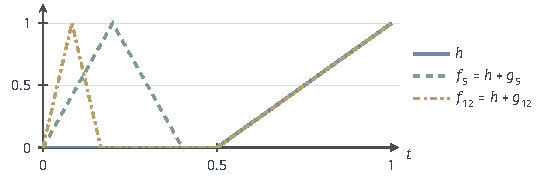
\includegraphics[width=92.8mm]{figures/02-abstract-mathematics/03-function-spaces/tikz/c2-weak-norm-drop/figure.pdf}
  \caption{一致范数下弱收敛加范数收敛不推出强收敛。$h(t)=\max(0,2t-1)$（蓝），$f_n=h+g_n$，其中$g_n$是支撑在$[0,2/n]$、峰值为$1$的尖峰；图中为$n=5$（绿虚线）与$n=12$（黄点划线）。$\|f_n\|_\infty=\|h\|_\infty=1$，$f_n\rightharpoonup h$，但$\|f_n-h\|_\infty=1$。}
  \label{fig:lfo-weak-norm-drop}
\end{figure}

\subsection{Hilbert空间中的弱收敛子列}
\label{sec:lfo-weak-subsequence}

有限维中，有界序列总有收敛子列；无限维中$e_n$说明这对范数收敛不成立。弱收敛的要求更低，本小节证明在Hilbert空间中它恢复了这个性质。

\begin{theorem}[Hilbert空间中的弱子列]
\label{thm:lfo-weak-subsequence}
Hilbert空间中的每个有界序列都有弱收敛的子列。
\end{theorem}

先在可分情形用标准正交基把问题化为系数列，再推广到一般情形。

\begin{proof}
设$\|x_n\|\leq C$。

\emph{第一步：逐个系数抽子列。}先设$H$可分，取标准正交基$(e_k)$，记系数$c_{n,k}=\langle e_k,x_n\rangle$，$|c_{n,k}|\leq C$。有界数列有收敛子列：先从$(x_n)$中抽子列使第$1$个系数收敛，再从中抽子列使第$2$个系数收敛，如此继续。取第$j$个子列的第$j$项组成对角子列$(x_{n_j})$，它从某项起是每个子列的子列，所以对每个$k$，$c_{n_j,k}\to a_k$。

\emph{第二步：极限系数平方可和。}对任意有限的$K$，$\sum_{k\leq K}|a_k|^2=\lim_j\sum_{k\leq K}|c_{n_j,k}|^2\leq C^2$，后一个不等式是Bessel不等式。令$K\to\infty$，$\sum_k|a_k|^2\leq C^2$，所以$x=\sum_ka_ke_k\in H$，$\|x\|\leq C$。

\emph{第三步：对所有方向收敛。}任取$y\in H$及$\varepsilon>0$，取$K$使$\|y-P_Ky\|<\varepsilon$，其中$P_K$是到前$K$个基向量的投影。分解
\[
 \langle y,x_{n_j}-x\rangle=\langle P_Ky,x_{n_j}-x\rangle+\langle y-P_Ky,x_{n_j}-x\rangle .
\]
第一项是有限个系数之差的线性组合，随$j\to\infty$趋于零；第二项不超过$\varepsilon\cdot2C$。所以$\limsup_j|\langle y,x_{n_j}-x\rangle|\leq2C\varepsilon$，由$\varepsilon$任意得$x_{n_j}\rightharpoonup x$。

\emph{第四步：一般Hilbert空间。}令$M$为$\{x_n\}$的闭线性张成。有理系数（复情形为实部虚部都有理）的有限线性组合在$M$中稠密，所以$M$可分，对$M$应用前三步得到子列与$x\in M$，使对一切$y\in M$弱收敛成立。对一般的$y\in H$，写$y=P_My+(y-P_My)$，后者与$M$正交，从而与每个$x_n$及$x$的内积都是零，故$\langle y,x_{n_j}\rangle=\langle P_My,x_{n_j}\rangle\to\langle P_My,x\rangle=\langle y,x\rangle$。
\end{proof}

\paragraph{坐标收敛还不够}
第三步不能省略：逐个系数收敛本身并不等于弱收敛。$x_n=n\,e_n$的每个坐标都最终为零，坐标逐点收敛到零向量，但取$y_k=1/k$，$\langle y,x_n\rangle=1$不趋于零。证明中让有限截断与尾项估计配合的，是序列的统一界$C$；有界性加坐标收敛才推出弱收敛。

\paragraph{弱子列不是范数紧性}
定理只保证弱收敛的子列。单位向量$e_n$本身就弱收敛到零，但没有范数收敛的子列，所以单位球在范数下不紧。弱极限也不必保留序列满足的约束：每个$e_n$都在单位球面$\{\|x\|=1\}$上，弱极限$0$却不在。哪些约束集在弱极限下封闭（例如闭凸集），以及由此得到的极小值存在性，属于优化问题中的存在性讨论，与第~\ref{sec:lfo-finite-observations}节末提到的拟合问题一样留给卷三的优化部分。

\subsection{反射空间的弱紧性（补充）}
\label{sec:lfo-reflexive}

上一小节的证明利用了标准正交基。离开Hilbert空间，有界序列是否仍有弱收敛子列？答案取决于空间与它的二次对偶的关系。

\paragraph{自然嵌入与反射}
每个$x\in X$都给出对偶空间上的一个读数：$(Jx)(L)=L(x)$，$L\in X^*$。$J:X\to X^{**}$线性，由定理~\ref{thm:lfo-norming-functional}，$\|Jx\|=\sup_{\|L\|\leq1}|L(x)|=\|x\|$，所以$J$是保范数的嵌入，称为\term{自然嵌入}（canonical embedding）。若$J$是满射，即$X^{**}$的每个元素都是某个$x$对应的读数，则称$X$为\term{反射空间}（reflexive space）。反射空间必然完备，因为$X^{**}$作为对偶空间是完备的。

有限维空间和Hilbert空间都是反射的：后者用两次Riesz表示即可验证。对$1<p<\infty$，由定理~\ref{thm:lfo-lp-dual}，$(L^p)^*\cong L^q$，$(L^q)^*\cong L^p$，逐层追踪对应关系可以验证合成后正是$J$，所以$L^p$是反射的。第~\ref{sec:lfo-lp-dual}节的端点讨论则表明$\ell^1$不是反射的：它的二次对偶是$(\ell^\infty)^*$，严格大于$\ell^1$。

\begin{theorem}[反射空间的弱紧性]
\label{thm:lfo-reflexive-compact}
设$X$是反射Banach空间。则$X$的闭单位球在弱拓扑下紧，并且$X$中每个有界序列都有弱收敛的子列。
\end{theorem}

\paragraph{为什么要单独陈述序列结论}
弱拓扑一般不能由度量给出，所以第~\ref{sec:metric-compact-sequential-tests}节中“紧等价于序列紧”的结论不能直接套用；从紧性推出序列结论需要另一个定理（Eberlein--Šmulian定理）。对序列结论，可以给一个直接的证明思路：令$Y$为序列的闭线性张成，它可分且反射；由$Y^{**}=J(Y)$可分可推出$Y^*$可分；在$Y^*$的可数稠密集上逐个对角化，得到使每个读数$L(x_{n_j})$都收敛的子列；极限读数是$Y^{**}$的元素，由反射性对应某个$x\in Y$；最后用Hahn--Banach定理把$X^*$中的读数限制到$Y$上，得到$x_{n_j}\rightharpoonup x$。一般证明属于补充。

\paragraph{$L^1$中质量集中的序列}
有界性在非反射空间中不足以保证弱子列。在$L^1(0,1)$中令$f_n=n\mathbf 1_{(0,1/n)}$，$\|f_n\|_1=1$。设某个子列$f_{n_j}\rightharpoonup f\in L^1$。对任意$0<a<1$，取读数$g=\mathbf 1_{(a,1)}\in L^\infty$；当$n_j>1/a$时$\int_a^1f_{n_j}\,dt=0$，所以$\int_a^1f\,dt=0$。对一切$a$成立，相减得$f$在每个区间$(a,b)\subset(0,1)$上积分为零，从而$f=0$几乎处处。但取读数$g\equiv1$，$\int_0^1f_{n_j}\,dt=1$，又得$\int_0^1f\,dt=1$，矛盾。

图~\ref{fig:lfo-escaping-mass}画出了这一列：质量始终为$1$，却向左端点越挤越窄。远离零点的读数（灰色区域）看到的是零，整体积分看到的却是一。极限对象应当是Dirac测度$\delta_0$，它不是$L^1$中的函数，这一列在$L^1$中找不到弱极限。所以第~\ref{sec:lfo-weak-subsequence}节和本小节的结论不能无条件推广到$L^1$或$L^\infty$。

\begin{figure}[!htb]
  \centering
  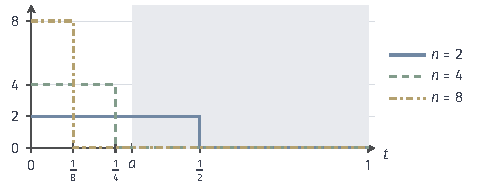
\includegraphics[width=80.8mm]{figures/02-abstract-mathematics/03-function-spaces/tikz/c2-escaping-mass/figure.pdf}
  \caption{$L^1(0,1)$中有界但没有弱收敛子列的序列$f_n=n\mathbf 1_{(0,1/n)}$，图中$n=2,4,8$。每个$f_n$的积分都为$1$；灰色区域是读数$\mathbf 1_{(a,1)}$（$a=0.3$）的支撑，$n>1/a$后在该区域上的积分为零。远离原点的读数迫使候选极限几乎处处为零，整体积分却保持为$1$，二者不能同时满足。}
  \label{fig:lfo-escaping-mass}
\end{figure}

\subsection{对偶空间的弱星紧性（补充）}
\label{sec:lfo-weak-star}

上面的$f_n\,dt$若看成$C([0,1])$上的读数，确实“收敛”到$\delta_0$：对每个连续$u$，$\int_0^1uf_n\,dt\to u(0)$。这提示我们，当变化的对象本身是读数时，可以只用原空间的元素去测试它们。

\begin{definition}[弱星收敛]
\label{def:lfo-weak-star}
设$X$是赋范空间，$L_n,L\in X^*$。若对每个$x\in X$都有$L_n(x)\to L(x)$，则称$L_n$\term{弱星收敛}（weak-star convergence）到$L$，记为$L_n\overset{*}{\rightharpoonup}L$。
\end{definition}

$X^*$本身是Banach空间，它也有自己的弱收敛，测试对象是$X^{**}$的全部元素；弱星收敛只用自然嵌入的像$J(X)\subset X^{**}$测试，要求更少。所以在$X^*$中，弱收敛蕴含弱星收敛，$X$反射时二者一致。

\paragraph{Banach--Alaoglu定理}
弱星收敛的好处是紧性在任何对偶空间中都成立，不需要反射性，这就是\term{Banach--Alaoglu定理}（Banach--Alaoglu theorem）。

\begin{theorem}[Banach--Alaoglu]
\label{thm:lfo-banach-alaoglu}
设$X$是赋范空间。则$X^*$的闭单位球在弱星拓扑下紧。
\end{theorem}

这里的紧性所对应的测试对象是原空间$X$。一般证明把单位球嵌入乘积空间$\prod_{x\in X}[-\|x\|,\|x\|]$，再用Tychonoff定理，属于补充。和反射空间一样，一般的弱星紧性不直接给出序列结论；下面在前对偶$X$可分的条件下给出直接证明。

\begin{theorem}[可分前对偶下的弱星子列]
\label{thm:lfo-weak-star-sequential}
设$X$是可分赋范空间。则$X^*$中每个有界序列都有弱星收敛的子列。
\end{theorem}

\begin{proof}
设$\|L_n\|\leq C$，$\{z_k\}$是$X$的可数稠密子集。对每个$k$，$(L_n(z_k))_n$是有界数列；与定理~\ref{thm:lfo-weak-subsequence}的第一步相同，逐个$k$抽子列再取对角，得到子列$(L_{n_j})$，使$L_{n_j}(z_k)$对每个$k$都收敛。

对一般的$x\in X$及$\varepsilon>0$，取$z_k$使$\|x-z_k\|<\varepsilon$，则
\[
 \begin{aligned}
 |L_{n_i}(x)-L_{n_j}(x)|
 &\leq|L_{n_i}(x-z_k)|+|L_{n_i}(z_k)-L_{n_j}(z_k)|+|L_{n_j}(z_k-x)|\\
 &\leq2C\varepsilon+|L_{n_i}(z_k)-L_{n_j}(z_k)| .
 \end{aligned}
\]
最后一项在$i,j$充分大时小于$\varepsilon$，所以$(L_{n_j}(x))$是Cauchy数列，极限记为$L(x)$。$L$是线性的，且$|L(x)|\leq C\|x\|$，故$L\in X^*$，$L_{n_j}\overset{*}{\rightharpoonup}L$。
\end{proof}

统一的范数界$C$在证明中起了关键作用：它把可数个测试点上的收敛推广到所有测试点。可分性则保证只需对可数个测试点对角化。

\paragraph{$L^\infty$中的振荡}
$L^\infty(0,1)$是可分空间$L^1(0,1)$的对偶，所以其中的有界序列有弱星收敛的子列。取$g_n(t)=\operatorname{sgn}(\sin(2\pi nt))$，它在$2n$个等长小区间上交替取$\pm1$，$\|g_n\|_\infty=1$。对区间的示性函数$f=\mathbf 1_{(a,b)}$，$\int g_nf\,dt$只来自两端不完整的小区间，绝对值不超过$1/n$，趋于零；由线性对阶梯函数成立，再由阶梯函数在$L^1$中稠密及统一界$\|g_n\|_\infty=1$推广到一切$f\in L^1$。所以$g_n\overset{*}{\rightharpoonup}0$，而$\|g_n-g_m\|_\infty$不趋于零，序列不按范数收敛。

同样，$C([0,1])$可分，本小节开头的$f_n\,dt$作为$C([0,1])^*$中的有界序列弱星收敛到$\delta_0$。在$L^1$中找不到的极限，在更大的对偶空间$C([0,1])^*$中以测度的形式出现了。

\paragraph{可分性不能省}
若前对偶不可分，序列结论可以失效。$\ell^\infty$不可分；考虑其对偶中的读数$L_n(x)=x_n$，$\|L_n\|=1$。对任意子列$(L_{n_j})$，取$x\in\ell^\infty$使$x_{n_j}=(-1)^j$（其余坐标为零），则$L_{n_j}(x)=(-1)^j$不收敛。所以这个有界序列没有弱星收敛的子列，尽管Banach--Alaoglu定理仍保证单位球弱星紧。可分性必须写在序列结论之前。

% 第2章第5节：算子的伴随与空间分解（伴随算子、像与核、自伴与正算子及正交投影、条件期望的投影解释）。

\section{算子的伴随与空间分解}
\label{sec:lfo-adjoint}

本节回到Hilbert空间之间的一般算子。前两节说明，Hilbert空间中的每个连续读数都是一个方向；现在用这一点研究算子怎样把输出空间中的测试方向对应回输入空间，并由此回答两个问题：哪些输入方向在输出中完全看不见，哪些输出能被算子的像逼近。自伴与正性进一步刻画同一空间中的方向关系，正交投影和条件期望是最重要的例子。

\subsection{伴随算子}
\label{sec:lfo-adjoint-def}

\paragraph{把输出测试拉回输入}
设$H_1,H_2$是Hilbert空间，$A\in\mathcal B(H_1,H_2)$。固定输出空间中的方向$v\in H_2$，考察读数$u\mapsto\langle v,Au\rangle$：先把输入$u$送到输出空间，再用$v$去测试。它对$u$线性，且$|\langle v,Au\rangle|\leq\|v\|\,\|A\|\,\|u\|$，所以是$H_1$上的有界线性泛函。由Riesz表示定理，存在唯一的$w\in H_1$使$\langle v,Au\rangle=\langle w,u\rangle$对一切$u$成立。这个$w$随$v$而定，记为$A^*v$。

\begin{definition}[伴随算子]
\label{def:lfo-adjoint}
设$A\in\mathcal B(H_1,H_2)$。由
\begin{equation}
 \langle v,Au\rangle_{H_2}=\langle A^*v,u\rangle_{H_1}\qquad(u\in H_1,\ v\in H_2)
 \label{eq:lfo-adjoint}
\end{equation}
确定的映射$A^*:H_2\to H_1$称为$A$的\term{伴随}（adjoint）算子。
\end{definition}

伴随回答的问题是：用输出方向$v$测试$Au$，相当于在输入空间中用哪个方向测试$u$。它把测试方向从输出空间拉回输入空间，并不是从输出恢复输入。下面的移位算子会清楚地显示这一区别。

\begin{theorem}[伴随的基本性质]
\label{thm:lfo-adjoint-properties}
设$A,B\in\mathcal B(H_1,H_2)$，$C\in\mathcal B(H_2,H_3)$，$\alpha\in\mathbb F$。则$A^*\in\mathcal B(H_2,H_1)$，并且
\[
 \begin{aligned}
 &(A+B)^*=A^*+B^*,\quad(\alpha A)^*=\bar\alpha A^*,\quad(CA)^*=A^*C^*,\\
 &A^{**}=A,\quad\|A^*\|=\|A\|,\quad\|A^*A\|=\|A\|^2 .
 \end{aligned}
\]
\end{theorem}

\begin{proof}
\emph{线性。}对$v_1,v_2$及标量$\beta_1,\beta_2$，$\langle A^*(\beta_1v_1+\beta_2v_2),u\rangle=\langle\beta_1v_1+\beta_2v_2,Au\rangle=\bar\beta_1\langle A^*v_1,u\rangle+\bar\beta_2\langle A^*v_2,u\rangle=\langle\beta_1A^*v_1+\beta_2A^*v_2,u\rangle$，由Riesz表示的唯一性即得。和、数乘与复合的公式用同样的方式验证，例如$\langle v,CAu\rangle=\langle C^*v,Au\rangle=\langle A^*C^*v,u\rangle$；数乘中的共轭来自内积对第一个变量共轭线性。

\emph{有界与范数。}由$\|A^*v\|^2=\langle A^*v,A^*v\rangle=\langle v,AA^*v\rangle\leq\|v\|\,\|A\|\,\|A^*v\|$得$\|A^*v\|\leq\|A\|\,\|v\|$，即$\|A^*\|\leq\|A\|$。对$A^*$的伴随求共轭可知$\langle u,A^*v\rangle=\langle Au,v\rangle$，所以$A^{**}=A$，再用一次刚才的不等式得$\|A\|=\|A^{**}\|\leq\|A^*\|$。

\emph{$\|A^*A\|=\|A\|^2$。}一方面$\|A^*A\|\leq\|A^*\|\,\|A\|=\|A\|^2$；另一方面对单位向量$u$，$\|Au\|^2=\langle u,A^*Au\rangle\leq\|A^*A\|$，取上确界得$\|A\|^2\leq\|A^*A\|$。
\end{proof}

\paragraph{矩阵与积分核}
在$\mathbb F^n$与$\mathbb F^m$上配标准内积，矩阵$\bm A$的伴随就是共轭转置$\bm A^{\mathsf H}$，实情形即转置。函数空间中，最常见的例子是积分算子。在$L^2(0,1)$上取$(Vu)(s)=\int_0^su(t)\,dt$，即从$0$累积到$s$。对$v\in L^2(0,1)$，由Fubini定理（定理~\ref{thm:integral-fubini}，被积函数在三角形区域上可积）交换积分次序：
\[
 \langle v,Vu\rangle=\int_0^1\overline{v(s)}\int_0^su(t)\,dt\,ds=\int_0^1\Bigl(\int_t^1\overline{v(s)}\,ds\Bigr)u(t)\,dt ,
\]
所以$(V^*v)(t)=\int_t^1v(s)\,ds$，即从$t$累积到$1$。用$u=v=1$核对：$\langle1,V1\rangle=\int_0^1s\,ds=1/2$，$V^*1=1-t$，$\langle V^*1,1\rangle=\int_0^1(1-t)\,dt=1/2$。一般地，核为$k(s,t)$的积分算子，其伴随的核是$\overline{k(t,s)}$，第~\ref{sec:ose-kernel-symmetry}节将系统讨论。

\paragraph{伴随不是逆}
在$\ell^2$上，右移$S(x_1,x_2,\ldots)=(0,x_1,x_2,\ldots)$的伴随是左移$S^*(y_1,y_2,\ldots)=(y_2,y_3,\ldots)$：逐项核对$\langle y,Sx\rangle=\sum_{k\geq1}\bar y_{k+1}x_k=\langle S^*y,x\rangle$。于是$S^*S=I$，左移撤销了右移；但$SS^*(y_1,y_2,\ldots)=(0,y_2,y_3,\ldots)$，第一个坐标被抹掉了，$SS^*\neq I$。$S$保持长度，不丢失信息，但它的像缺少$e_1$方向，所以$S^*$只是左逆。对一般算子，$A^*$连左逆都不是：零算子的伴随是零算子。

\paragraph{Banach空间中的转置}
没有内积时，仍然可以把输出读数拉回输入。对$A\in\mathcal B(X,Y)$，令$A'L=L\circ A$，$L\in Y^*$，得到\term{转置算子}（transpose operator）$A':Y^*\to X^*$。由定理~\ref{thm:lfo-norming-functional}可以证明$\|A'\|=\|A\|$。转置作用在对偶空间之间；只有在Hilbert空间中借助Riesz对应把读数换成向量，才能把它写成作用在$H_2$与$H_1$之间的伴随$A^*$。

\subsection{像空间与零空间}
\label{sec:lfo-range-kernel}

\paragraph{正交关系}
伴随的定义式~\eqref{eq:lfo-adjoint}把“输出与$Au$正交”翻译成输入空间中的条件。记$\operatorname{Ran}A=\{Au:u\in H_1\}$为像，$\ker A=\{u:Au=0\}$为核。

\begin{theorem}[像与核的正交关系]
\label{thm:lfo-range-kernel}
设$A\in\mathcal B(H_1,H_2)$。则
\begin{equation}
 (\operatorname{Ran}A)^\perp=\ker A^*,\qquad\overline{\operatorname{Ran}A}=(\ker A^*)^\perp ,
 \label{eq:lfo-range-kernel}
\end{equation}
交换$A$与$A^*$的角色，又有$(\operatorname{Ran}A^*)^\perp=\ker A$与$\overline{\operatorname{Ran}A^*}=(\ker A)^\perp$。
\end{theorem}

\begin{proof}
$y\in(\operatorname{Ran}A)^\perp$，当且仅当对一切$u$有$\langle y,Au\rangle=0$，即$\langle A^*y,u\rangle=0$；取$u=A^*y$可知这等价于$A^*y=0$。这证明了第一个等式。

对第二个等式，只需说明线性子空间$M$满足$(M^\perp)^\perp=\overline M$，再取$M=\operatorname{Ran}A$。显然$M\subset(M^\perp)^\perp$，后者是闭集，所以$\overline M\subset(M^\perp)^\perp$。反过来，设$y\in(M^\perp)^\perp$，由第~\ref{sec:fs-projection}节的正交分解$y=P_{\overline M}y+z$，$z\in(\overline M)^\perp=M^\perp$；而$y$与$P_{\overline M}y$都与$z$正交，所以$\|z\|^2=\langle z,y-P_{\overline M}y\rangle=0$，$y\in\overline M$。其余两式把$A$换成$A^*$并用$A^{**}=A$即得。
\end{proof}

由此得到两个空间的正交分解：
\[
 H_1=\ker A\oplus\overline{\operatorname{Ran}A^*},\qquad H_2=\ker A^*\oplus\overline{\operatorname{Ran}A} .
\]
图~\ref{fig:lfo-four-subspaces}把这四个子空间放在一起。$\ker A$中的输入方向在输出中完全看不见，加到任何输入上都不改变输出；$\overline{\operatorname{Ran}A}$是能被输出逼近的方向；$\ker A^*$中的输出方向与一切输出正交，任何输入都到达不了。这是有限维中“四个基本子空间”在Hilbert空间中的形式，区别在于像必须取闭包。

\begin{figure}[!htb]
  \centering
  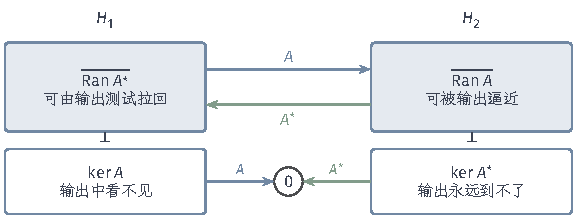
\includegraphics[width=97.7mm]{figures/02-abstract-mathematics/03-function-spaces/tikz/c2-four-subspaces/figure.pdf}
  \caption{伴随与像、核的正交关系。输入空间分解为$H_1=\ker A\oplus\overline{\operatorname{Ran}A^*}$，输出空间分解为$H_2=\ker A^*\oplus\overline{\operatorname{Ran}A}$。$A$把$\ker A$送到零，其余输入的输出都落在$\operatorname{Ran}A$中；$A^*$把$\ker A^*$送到零。无限维中像未必闭合，正交关系只确定像的闭包。}
  \label{fig:lfo-four-subspaces}
\end{figure}

\paragraph{累积算子的像}
以上面的$V$为例。若$V^*v=0$，则$\int_t^1v(s)\,ds=0$对一切$t$成立，于是$v$在每个区间$(t,1)$上积分为零，从而$v=0$几乎处处，$\ker V^*=\{0\}$。由式~\eqref{eq:lfo-range-kernel}，$\operatorname{Ran}V$在$L^2(0,1)$中稠密。但$\operatorname{Ran}V$中的函数都是连续的，阶跃函数$\mathbf 1_{(1/2,1)}$不在其中，所以$\operatorname{Ran}V\neq L^2(0,1)$：像稠密而不闭。

\paragraph{像稠密不闭的数列例子}
在$\ell^2$上令$A(x_n)=(x_n/n)$，即第$n$个坐标乘以$1/n$。它是自伴的（$A^*=A$），单射，所以$\ker A^*=\{0\}$，像在$\ell^2$中稠密。考察$y=(1/n)$，由$\sum_n1/n^2<\infty$知$y\in\ell^2$。若$Ax=y$，逐个坐标比较得$x_n=1$，这个唯一的形式逆像不是平方可和的，所以$y\notin\operatorname{Ran}A$。

截断形式逆像可以看清发生了什么。令$x^{(N)}=(1,\ldots,1,0,0,\ldots)$，前$N$个坐标为$1$。则
\[
 \|Ax^{(N)}-y\|^2=\sum_{n>N}\frac1{n^2}\longrightarrow0,\qquad\|x^{(N)}\|=\sqrt N\longrightarrow\infty .
\]
图~\ref{fig:lfo-dense-range}显示：残差随$N$增大趋于零，说明$y$在像的闭包中；为了取得这些越来越好的近似，输入的范数却无限增大。输出上越来越小的修正需要越来越大的输入，这正是第~\ref{sec:lfo-inverse}节要讨论的不稳定性。

\begin{figure}[!htb]
  \centering
  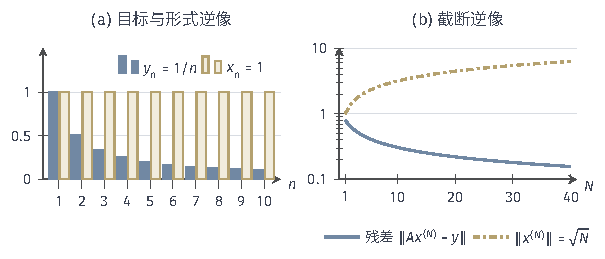
\includegraphics[width=102.5mm]{figures/02-abstract-mathematics/03-function-spaces/tikz/c2-dense-range/figure.pdf}
  \caption{$\ell^2$上$A(x_n)=(x_n/n)$的像稠密而不闭。(a)~目标$y_n=1/n$（蓝）平方可和，但唯一的形式逆像$x_n=1$（黄）不平方可和；(b)~截断逆像$x^{(N)}$的残差$\|Ax^{(N)}-y\|$（蓝）趋于零，范数$\|x^{(N)}\|=\sqrt N$（黄点划线）趋于无穷，纵轴为对数刻度。}
  \label{fig:lfo-dense-range}
\end{figure}

\paragraph{正交条件只确定像的闭包}
这个例子划出了正交关系的边界。$y\perp\ker A^*$只能保证$y$在像的闭包中，不能保证方程$Ax=y$精确可解。只有已经知道$\operatorname{Ran}A$闭合时，才有$\operatorname{Ran}A=(\ker A^*)^\perp$，此时$Ax=y$可解当且仅当$y$与$\ker A^*$正交。第~\ref{chap:operator-spectra-equations}章的Fredholm理论和第一类方程都会反复使用这一边界。

\subsection{自伴、正算子与正交投影}
\label{sec:lfo-self-adjoint}

\paragraph{自伴与正算子}
当输入和输出在同一个Hilbert空间$H$中时，可以比较$A$与$A^*$。若$A=A^*$，即$\langle v,Au\rangle=\langle Av,u\rangle$对一切$u,v$成立，则称$A$为\term{自伴}（self-adjoint）算子。自伴算子的二次型$\langle x,Ax\rangle$总是实数，因为它等于自身的共轭$\langle Ax,x\rangle$。

\begin{definition}[正算子]
\label{def:lfo-positive-operator}
设$A\in\mathcal B(H)$自伴。若$\langle x,Ax\rangle\geq0$对一切$x\in H$成立，则称$A$为\term{正算子}（positive operator），记为$A\geq0$。
\end{definition}

定义中要求先自伴，是因为在实空间中二次型非负并不能推出对称：平面上逆时针旋转$90^\circ$的矩阵满足$\bm x^{\top}\bm A\bm x=0$，却不对称。最基本的正算子是$A^*A$：$\langle x,A^*Ax\rangle=\|Ax\|^2\geq0$。

\paragraph{三种强度的正性}
对自伴算子，下面三个条件依次加强：（i）$\langle x,Ax\rangle\geq0$对一切$x$成立；（ii）$\langle x,Ax\rangle>0$对一切$x\neq0$成立；（iii）存在常数$c>0$，使$\langle x,Ax\rangle\geq c\|x\|^2$对一切$x$成立，此时称$A$具有\term{强制性}（coercivity）。有限维中（ii）与（iii）等价，因为单位球面紧，连续函数在其上取到正的最小值；无限维中不再如此。上一小节的$A(x_n)=(x_n/n)$满足（ii），因为$\langle x,Ax\rangle=\sum_n|x_n|^2/n>0$；但$\langle e_n,Ae_n\rangle=1/n\to0$，没有统一的下界$c$。逐方向严格为正，不能当作统一下界。

统一下界对逆向恢复有直接意义。若$A$自伴且强制，则由Cauchy--Schwarz不等式$c\|x\|^2\leq\langle x,Ax\rangle\leq\|x\|\,\|Ax\|$，得$\|Ax\|\geq c\|x\|$。由此$A$单射；像是闭的，因为若$Ax_n\to y$，则$\|x_n-x_m\|\leq c^{-1}\|Ax_n-Ax_m\|$，$(x_n)$是Cauchy列，极限$x$满足$Ax=y$；又$\ker A^*=\ker A=\{0\}$，由定理~\ref{thm:lfo-range-kernel}像稠密。像既闭又稠密，所以$A$是双射，且$\|A^{-1}\|\leq1/c$。只有逐方向严格正的算子则可能像不闭，正如$(x_n/n)$。

\paragraph{正交投影的算子刻画}
第~\ref{sec:fs-projection}节从最近点问题得到了正交投影$P_M$。现在用算子性质刻画它。

\begin{theorem}[正交投影的刻画]
\label{thm:lfo-orthogonal-projection}
设$P\in\mathcal B(H)$。则$P$是到某个闭子空间的正交投影，当且仅当$P^2=P$且$P^*=P$。此时该子空间为$M=\operatorname{Ran}P$，且$P\geq0$，$\|P\|\leq1$。
\end{theorem}

\begin{proof}
若$P=P_M$，则$P^2=P$是因为$M$中元素的投影是它自己。对任意$x,z$，$\langle z,Px\rangle=\langle Pz+(z-Pz),Px\rangle=\langle Pz,Px\rangle$，因为$z-Pz\perp M$；同理$\langle Pz,x\rangle=\langle Pz,Px\rangle$，所以$P^*=P$。

反过来，设$P^2=P=P^*$。令$M=\operatorname{Ran}P$。由$P^2=P$，$M=\ker(I-P)$，是闭子空间。对任意$x$，$Px\in M$，而$x-Px\in\ker P$；由定理~\ref{thm:lfo-range-kernel}，$\ker P=\ker P^*=(\operatorname{Ran}P)^\perp=M^\perp$。所以$x=Px+(x-Px)$恰是$x$沿$M\oplus M^\perp$的分解，$Px=P_Mx$。最后，$\langle x,Px\rangle=\langle Px,Px\rangle=\|Px\|^2\geq0$，且$\|Px\|^2\leq\|Px\|^2+\|x-Px\|^2=\|x\|^2$。
\end{proof}

只满足$P^2=P$的算子称为投影，它把空间分解为$\operatorname{Ran}P\oplus\ker P$，但两部分不一定正交，这样的投影称为\term{斜投影}（oblique projection）。图~\ref{fig:lfo-projections}(a)中，$P(x_1,x_2)=(x_1+x_2,0)$满足$P^2=P$，像是横轴，核是直线$x_1+x_2=0$。点$\bm x=(0.6,0.9)$被沿核的方向送到$(1.5,0)$，比正交投影$(0.6,0)$离$\bm x$更远。斜投影可以放大长度：$\|P\|=\sqrt2>1$，在方向$(1,1)/\sqrt2$上取到。

\begin{figure}[!htb]
  \centering
  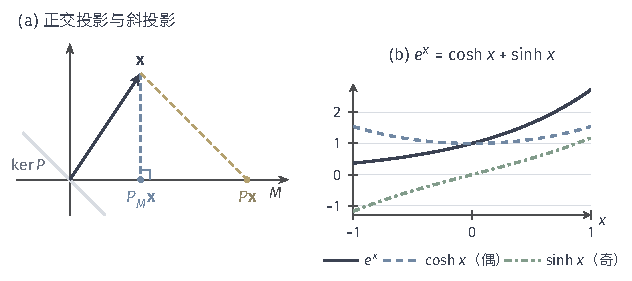
\includegraphics[width=107.0mm]{figures/02-abstract-mathematics/03-function-spaces/tikz/c2-projections/figure.pdf}
  \caption{正交投影与斜投影、偶部分与奇部分。(a)~平面中$\bm x=(0.6,0.9)$到横轴$M$的正交投影为$(0.6,0)$（蓝），残差与$M$垂直；斜投影$P(x_1,x_2)=(x_1+x_2,0)$沿核$x_1+x_2=0$（灰线）把$\bm x$送到$(1.5,0)$（黄），残差不与$M$垂直；(b)~$L^2(-1,1)$中$e^x$分解为偶部分$\cosh x$（蓝虚线）与奇部分$\sinh x$（绿点划线），两部分正交。}
  \label{fig:lfo-projections}
\end{figure}

\paragraph{偶函数投影}
在$L^2(-1,1)$上令
\[
 (Pu)(x)=\frac{u(x)+u(-x)}{2}.
\]
直接验证$P^2=P$。自伴性来自变量替换$x\mapsto-x$保持Lebesgue测度：$\int_{-1}^1\overline{v(x)}u(-x)\,dx=\int_{-1}^1\overline{v(-x)}u(x)\,dx$，于是$\langle v,Pu\rangle=\langle Pv,u\rangle$。由定理~\ref{thm:lfo-orthogonal-projection}，$P$是正交投影，像是偶函数子空间，核是奇函数子空间，两者正交。

以$u(x)=e^x$为例，$Pu=\cosh x$，$(I-P)u=\sinh x$，如图~\ref{fig:lfo-projections}(b)。正交性可以直接核对：$\cosh x\sinh x$是奇函数，在$[-1,1]$上积分为零。勾股恒等式也可以复算：
\[
 \begin{aligned}
 &\|e^x\|^2=\int_{-1}^1e^{2x}\,dx=\sinh2\approx3.627,\\
 &\|\cosh x\|^2=1+\tfrac12\sinh2\approx2.813,\qquad
 \|\sinh x\|^2=\tfrac12\sinh2-1\approx0.813 ,
 \end{aligned}
\]
后两者之和正是前者。若把区间换成不对称的$[-1,2]$，或把测度换成不对称的权重，替换$x\mapsto-x$不再保持内积，同一公式就不再给出正交投影。

\paragraph{有限群平均（补充）}
偶函数投影是对二元群$\{x,-x\}$求平均。一般地，设有限群$G$由保持测度的可逆变换组成，令$(Pu)(x)=|G|^{-1}\sum_{g\in G}u(g(x))$。同样的变量替换说明$P$自伴，群的结构说明$P^2=P$，所以$P$是到$G$不变函数子空间的正交投影。这只是一个空间分解的事实；把数据或模型投影到不变子空间是否改善某个统计任务，需要另外的分析，不能由投影性质直接推出。

\subsection{条件期望的投影解释}
\label{sec:lfo-conditional-expectation}

正交投影最重要的概率实例是条件期望。本小节只补充它的空间解释，所用的条件期望定义与性质先就地写明。

\paragraph{所用的定义与性质}
设$(\Omega,\mathcal F,\mathbb P)$是概率空间，$\mathcal G\subset\mathcal F$是子$\sigma$代数。为避免与空间记号$X$冲突，本小节用$Z$表示随机变量，并只考虑实值情形。对可积的$Z$，\term{条件期望}（conditional expectation）$\mathbb E[Z\mid\mathcal G]$是满足
\begin{equation}
 \mathbb E\bigl[\mathbb E[Z\mid\mathcal G]\,\mathbf 1_A\bigr]=\mathbb E[Z\mathbf 1_A]\qquad(A\in\mathcal G)
 \label{eq:lfo-conditional-expectation}
\end{equation}
的$\mathcal G$可测可积函数，在几乎处处相等的意义下唯一。它的存在性由Radon--Nikodym定理给出，具体做法是取$\mathcal G$上测度$G\mapsto\int_G Z\,d\mathbb P$关于$\mathbb P|_{\mathcal G}$的密度。下面还要用到两个标准性质：条件期望是线性的；条件Jensen不等式给出$(\mathbb E[Z\mid\mathcal G])^2\leq\mathbb E[Z^2\mid\mathcal G]$几乎处处成立。这些性质的系统建立属于第~\ref{part:probability-spaces}部分；离散与有密度情形下的初等版本可参考\BookChapterRef{chap:random-vectors}{卷一“随机向量与联合分布”章}。

\paragraph{$\mathcal G$可测元素组成闭子空间}
令$L^2(\mathcal G)$为$L^2(\Omega,\mathcal F,\mathbb P)$中有$\mathcal G$可测代表的等价类全体，它是线性子空间。它是闭的：设$Z_n\in L^2(\mathcal G)$且$Z_n\to Z$于$L^2$，取各$Z_n$的$\mathcal G$可测代表；由第~\ref{sec:fs-convergence-modes}节，可抽子列$Z_{n_k}\to Z$几乎处处。令$W=\limsup_kZ_{n_k}$（在其取有限值处，其余处取零），它作为$\mathcal G$可测函数的上极限是$\mathcal G$可测的，并且几乎处处等于$Z$，所以$Z\in L^2(\mathcal G)$。这里取上极限而不是直接修改零测集，是为了避免例外零测集本身不属于$\mathcal G$。

\paragraph{条件期望在这个子空间中}
设$Z\in L^2$，记$W=\mathbb E[Z\mid\mathcal G]$。由条件Jensen不等式并对式~\eqref{eq:lfo-conditional-expectation}取$A=\Omega$的形式，
\[
 \mathbb E[W^2]\leq\mathbb E\bigl[\mathbb E[Z^2\mid\mathcal G]\bigr]=\mathbb E[Z^2]<\infty ,
\]
所以$W\in L^2(\mathcal G)$，并且$\|W\|_2\leq\|Z\|_2$。

\paragraph{误差与子空间正交}
接下来验证$Z-W$与$L^2(\mathcal G)$中的每个元素正交。式~\eqref{eq:lfo-conditional-expectation}说明对示性函数$V=\mathbf 1_A$（$A\in\mathcal G$）有$\mathbb E[(Z-W)V]=0$；由线性，对$\mathcal G$可测的简单函数也成立；有界$\mathcal G$可测函数是这类简单函数的一致极限，而$Z-W$可积，所以由控制收敛定理推广到有界的$V$。最后，对一般的$V\in L^2(\mathcal G)$，令截断$V_k=V\mathbf 1_{\{|V|\leq k\}}$，它有界且$\mathcal G$可测；由控制收敛定理$\|V_k-V\|_2\to0$，而内积连续，所以
\[
 \mathbb E[(Z-W)V]=\lim_k\mathbb E[(Z-W)V_k]=0 .
\]

\begin{theorem}[条件期望是正交投影]
\label{thm:lfo-conditional-expectation-projection}
设$Z\in L^2(\Omega,\mathcal F,\mathbb P)$。则$\mathbb E[Z\mid\mathcal G]$是$Z$在闭子空间$L^2(\mathcal G)$上的正交投影。因此$Z\mapsto\mathbb E[Z\mid\mathcal G]$是$L^2$上范数为$1$的自伴正算子，并且
\[
 \mathbb E[(Z-\mathbb E[Z\mid\mathcal G])^2]=\min_{V\in L^2(\mathcal G)}\mathbb E[(Z-V)^2] .
\]
\end{theorem}

\begin{proof}
前面已经说明$W=\mathbb E[Z\mid\mathcal G]\in L^2(\mathcal G)$且$Z-W\perp L^2(\mathcal G)$。由第~\ref{sec:fs-projection}节，满足这两个条件的元素唯一，就是正交投影，并且它是子空间中离$Z$最近的元素。由定理~\ref{thm:lfo-orthogonal-projection}，它是自伴正算子；常数属于$L^2(\mathcal G)$且被保持不变，所以范数等于$1$。
\end{proof}

\paragraph{均方误差的分解}
由第~\ref{sec:fs-projection}节的勾股恒等式，
\[
 \mathbb E[Z^2]=\mathbb E\bigl[(\mathbb E[Z\mid\mathcal G])^2\bigr]+\mathbb E\bigl[(Z-\mathbb E[Z\mid\mathcal G])^2\bigr].
\]
第一项是只用$\mathcal G$中的信息能解释的部分，第二项是这些信息解释不了的残差。定理中的极小性说明，在一切只依赖$\mathcal G$信息的平方可积预测中，条件期望的均方误差最小。

\paragraph{嵌套信息与塔式性质}
若$\mathcal G_1\subset\mathcal G_2$，则$L^2(\mathcal G_1)\subset L^2(\mathcal G_2)$。记$P_1,P_2$为相应的投影，先投影到大的子空间、再投影到小的子空间，等于直接投影到小的子空间：$P_1P_2=P_1$；而小子空间中的元素在大子空间上的投影是它自己：$P_2P_1=P_1$。翻译成条件期望，就是塔式性质
\[
 \mathbb E\bigl[\mathbb E[Z\mid\mathcal G_2]\bigm|\mathcal G_1\bigr]=\mathbb E[Z\mid\mathcal G_1]=\mathbb E\bigl[\mathbb E[Z\mid\mathcal G_1]\bigm|\mathcal G_2\bigr].
\]
$P_1P_2=P_1$的验证只需一行：$P_2Z-Z\perp L^2(\mathcal G_2)\supset L^2(\mathcal G_1)$，所以$P_1(P_2Z)-P_1Z=P_1(P_2Z-Z)=0$。

\paragraph{分块平均的例子}
取$\Omega=[0,1)$，$\mathbb P$为均匀分布，$Z(\omega)=\omega^2$。设$\mathcal G_4$由四个区间$[k/4,(k+1)/4)$生成，$\mathcal G_2$由两半生成。对有限个区间生成的$\sigma$代数，$\mathcal G$可测函数就是在各区间上取常数的函数，式~\eqref{eq:lfo-conditional-expectation}要求条件期望在每个区间上等于$Z$的平均值：
\[
 \mathbb E[Z\mid\mathcal G_4]=4\int_{k/4}^{(k+1)/4}\omega^2\,d\omega=\frac{(k+1)^3-k^3}{48},
\]
即依次为$1/48,7/48,19/48,37/48$；而$\mathbb E[Z\mid\mathcal G_2]$在两半上分别为$1/12$与$7/12$。图~\ref{fig:lfo-conditional-expectation}画出了这两个阶梯函数。粗分块的值正是细分块的值两两再平均，例如$(1/48+7/48)/2=1/12$，这就是塔式性质。

\begin{figure}[!htb]
  \centering
  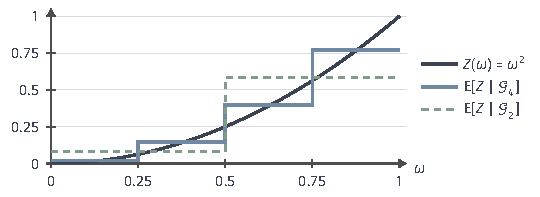
\includegraphics[width=91.4mm]{figures/02-abstract-mathematics/03-function-spaces/tikz/c2-conditional-expectation/figure.pdf}
  \caption{条件期望作为分块平均。$\Omega=[0,1)$上的均匀概率，$Z(\omega)=\omega^2$（黑）。$\mathcal G_4$由四个等长区间生成，$\mathbb E[Z\mid\mathcal G_4]$（蓝）在各区间上取$Z$的平均值$1/48,7/48,19/48,37/48$；$\mathcal G_2$由两半生成，$\mathbb E[Z\mid\mathcal G_2]$（绿虚线）取$1/12,7/12$，恰为细分块值的两两平均。}
  \label{fig:lfo-conditional-expectation}
\end{figure}

均方误差分解也可以复算。$\mathbb E[Z^2]=\int_0^1\omega^4\,d\omega=1/5$。四块时，$\mathbb E[W_4^2]=\frac14\cdot\frac{1+49+361+1369}{48^2}=\frac{1780}{9216}\approx0.1931$，残差约为$0.2-0.1931=0.0069$；两块时，$\mathbb E[W_2^2]=\frac12(\frac1{144}+\frac{49}{144})\approx0.1736$，残差约为$0.0264$。信息越细，子空间越大，投影离$Z$越近。两次投影之间的差$W_4-W_2$与$W_2$正交，$\mathbb E[(W_4-W_2)^2]=\frac{180}{9216}\approx0.0195$，恰好补足$0.1931-0.1736$。

本小节补充的是空间解释，没有重新建立条件期望的存在性。鞅、滤波与状态估计等以条件期望为基础的随机过程问题，可参考\BookChapterRef{chap:random-sequences-and-processes}{卷三“随机序列与随机过程”章}。

% 第2章第6节：逆算子与连续性判别（有界逆与开映射、闭图与图范数）。

\section{逆算子与连续性判别}
\label{sec:lfo-inverse}

由输出恢复输入，要同时满足三个不同的要求：给定的输出确实有原像（存在），原像只有一个（唯一），输出上的小误差只造成输入上的小误差（稳定）。有限维中，方阵可逆就同时满足这三条；无限维中它们会分离。本节先说明在完备性条件下，前两条自动推出第三条，再给出检验连续性的另一种方式。

\subsection{有界逆与开映射}
\label{sec:lfo-open-mapping}

\paragraph{唯一而不稳定}
回到第~\ref{sec:lfo-range-kernel}节的$A(x_n)=(x_n/n)$。它是单射，所以在像$\operatorname{Ran}A$上有唯一的形式逆$A^{-1}(y_n)=(ny_n)$。这个逆映射无界：$A^{-1}e_n=ne_n$，单位输出对应长度为$n$的输入。输出上$e_n/n$大小的误差，会在恢复时变成长度为$1$的输入误差。可解性与唯一性在这里都成立（在像上），稳定性却失败了。

\paragraph{完备空间之间的有界逆}
问题出在哪里？$A$并不是从$\ell^2$到$\ell^2$的双射，它的像只是$\ell^2$中稠密而不闭的子空间，按$\ell^2$范数不完备。下面的\term{有界逆定理}（bounded inverse theorem）说明，只要像是整个Banach空间，这种不稳定就不会发生。

\begin{theorem}[有界逆定理]
\label{thm:lfo-bounded-inverse}
设$X,Y$是Banach空间，$A\in\mathcal B(X,Y)$是双射。则$A^{-1}\in\mathcal B(Y,X)$。
\end{theorem}

定理中的值域是整个$Y$，而且$X,Y$都完备，这些条件都不能省。它说明，在Banach空间之间，有界的线性双射自动是稳定的；可解性加唯一性不足以推出稳定性的情形，一定是某个空间不完备或者像不是全空间。这个定理由下面更一般的\term{开映射定理}（open mapping theorem）推出。

\begin{theorem}[开映射定理]
\label{thm:lfo-open-mapping}
设$X,Y$是Banach空间，$A\in\mathcal B(X,Y)$是满射。则存在$\delta>0$，使$B_Y(0,\delta)\subset A\bigl(B_X(0,1)\bigr)$。等价地，每个$y\in Y$都有原像$x$满足$\|x\|\leq\delta^{-1}\|y\|$。
\end{theorem}

定理的内容是：满射不仅保证每个输出都有原像，还保证能选到一个范数受控的原像。证明分两步，第一步用Baire定理得到“输出球落在输入球的像的闭包中”，第二步用逐步修正残差去掉闭包。

\begin{proof}
记$B_r=B_X(0,r)$。

\emph{第一步：像的闭包含有输出球。}由满射，$Y=\bigcup_kA(B_k)=\bigcup_k\overline{A(B_k)}$。$Y$完备，由Baire定理（定理~\ref{thm:lfo-baire}），某个$\overline{A(B_k)}$包含开球$B_Y(y_0,r)$。对任意$\|y\|<r$，$y_0+y$与$y_0$都在$\overline{A(B_k)}$中，二者之差在$\overline{A(B_k)-A(B_k)}\subset\overline{A(B_{2k})}$中。所以$B_Y(0,r)\subset\overline{A(B_{2k})}$；按线性缩放，令$\eta=r/(2k)$，得
\[
 B_Y(0,\eta)\subset\overline{A(B_1)},\qquad\text{从而}\quad B_Y(0,\eta/2^j)\subset\overline{A(B_{2^{-j}})}\quad(j\geq0).
\]

\emph{第二步：逐步修正残差。}任取$\|y\|<\eta$。由第一步，存在$x_1\in B_1$使$\|y-Ax_1\|<\eta/2$。残差$y_1=y-Ax_1$落在$B_Y(0,\eta/2)$中，于是存在$x_2\in B_{1/2}$使$\|y_1-Ax_2\|<\eta/4$。如此继续，得到$x_k$满足
\[
 \|x_k\|<2^{1-k},\qquad\Bigl\|y-A\sum_{i\leq k}x_i\Bigr\|<\eta/2^k .
\]

\emph{第三步：用输入空间的完备性求和。}$\sum_k\|x_k\|<2$，部分和是$X$中的Cauchy列；$X$完备，所以$x=\sum_kx_k$存在，$\|x\|<2$。由$A$连续，$Ax=\lim_kA\sum_{i\leq k}x_i=y$。这说明$B_Y(0,\eta)\subset A(B_2)$，取$\delta=\eta/2$即得。
\end{proof}

第一步只得到闭包，不能直接说$B_Y(0,\eta)\subset A(B_1)$：闭包中的点只能被像逼近，未必是像。第二步的作用就是把“可以逼近”变成“可以达到”，代价是把输入球的半径从$1$放大到$2$，而这一步必须用到$X$的完备性。图~\ref{fig:lfo-open-mapping}画出了这个修正过程：每一步的修正量减半，输出残差也减半，输入的部分和收敛到真正的原像。

\begin{figure}[!htb]
  \centering
  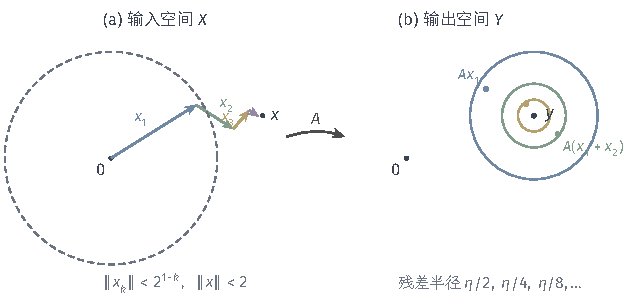
\includegraphics[width=107.4mm]{figures/02-abstract-mathematics/03-function-spaces/tikz/c2-open-mapping/figure.pdf}
  \caption{开映射定理证明中的残差修正（示意）。(b)~输出空间中，第一次近似$Ax_1$落在以$y$为心、半径$\eta/2$的球内（蓝圈），加上修正$x_2$后$A(x_1+x_2)$落入半径$\eta/4$的球（绿圈），依此类推；(a)~输入空间中修正量满足$\|x_k\|<2^{1-k}$，部分和收敛到原像$x$，$\|x\|<2$（虚线圆）。输入空间的完备性保证这一级数有极限。}
  \label{fig:lfo-open-mapping}
\end{figure}

\paragraph{由开映射推出有界逆}
设$A$是Banach空间之间的有界双射。由开映射定理，每个$y$有原像$x$满足$\|x\|\leq\delta^{-1}\|y\|$；单射使这个原像就是$A^{-1}y$，所以$\|A^{-1}y\|\leq\delta^{-1}\|y\|$，$A^{-1}$有界。这证明了定理~\ref{thm:lfo-bounded-inverse}。

\paragraph{等价范数}
有界逆定理的一个直接用途是比较范数。设线性空间$X$在两个范数$\|\cdot\|_a$、$\|\cdot\|_b$下都完备，且$\|x\|_a\leq C\|x\|_b$。则单位映射$I:(X,\|\cdot\|_b)\to(X,\|\cdot\|_a)$是有界双射，其逆也有界，于是存在$C'$使$\|x\|_b\leq C'\|x\|_a$：两个范数等价。若两个完备范数之间只有一个方向的控制，另一个方向的控制会自动出现。

\paragraph{像闭合与下有界}
有界逆定理还给出像闭合的判别。设$X,Y$是Banach空间，$A\in\mathcal B(X,Y)$单射。若$\operatorname{Ran}A$闭，则它是Banach空间，$A:X\to\operatorname{Ran}A$是有界双射，逆有界，于是存在$c>0$使
\begin{equation}
 \|Ax\|\geq c\|x\|\qquad(x\in X),
 \label{eq:lfo-bounded-below}
\end{equation}
这时称$A$\term{下有界}（bounded below）。反过来，若$A$下有界，第~\ref{sec:lfo-self-adjoint}节的论证说明$\operatorname{Ran}A$闭。所以对Banach空间之间的有界单射，像闭合当且仅当下有界。$A(x_n)=(x_n/n)$不满足式~\eqref{eq:lfo-bounded-below}，$\|Ae_n\|=1/n$，它的像也确实不闭。第~\ref{sec:ose-first-kind}节将看到，紧算子在无限维中永远不是下有界的，这正是第一类积分方程不稳定的根源。

\subsection{闭图与图范数（补充）}
\label{sec:lfo-closed-graph}

\paragraph{用极限检验连续性}
直接估计$\|Ax\|\leq C\|x\|$有时很困难。另一种思路是只检验一个较弱的条件：若输入$x_n\to x$，并且输出$Ax_n$也收敛到某个$y$，那么$y$是否必定等于$Ax$？这个条件只涉及输入、输出同时收敛的序列，不要求先证明输出收敛。把它写成几何语言：算子的图
\[
 \mathcal G(A)=\{(x,Ax):x\in D(A)\}\subset X\times Y
\]
在乘积范数$\|(x,y)\|=\|x\|+\|y\|$下是闭集。$X,Y$都完备时，$X\times Y$也是Banach空间。\term{闭图定理}（closed graph theorem）说明，对定义在整个完备空间上的算子，这个较弱的条件已经足够。

\begin{theorem}[闭图定理]
\label{thm:lfo-closed-graph}
设$X,Y$是Banach空间，$A:X\to Y$是定义在整个$X$上的线性算子。则$A$有界当且仅当$\mathcal G(A)$在$X\times Y$中闭。
\end{theorem}

\begin{proof}
若$A$有界，$x_n\to x$推出$Ax_n\to Ax$，所以$Ax_n\to y$时$y=Ax$，图闭。

反过来，设图闭。它是Banach空间$X\times Y$的闭线性子空间，因而本身是Banach空间。第一坐标投影$\pi(x,Ax)=x$是从$\mathcal G(A)$到$X$的有界线性双射（$\|x\|\leq\|(x,Ax)\|$；双射是因为$A$定义在整个$X$上，每个$x$恰好对应图中一点）。由有界逆定理，$\pi^{-1}$有界：存在$C$使$\|x\|+\|Ax\|\leq C\|x\|$，于是$\|Ax\|\leq C\|x\|$。
\end{proof}

\paragraph{处处有定义的对称算子有界}
闭图定理的一个漂亮应用：设$A:H\to H$是定义在整个Hilbert空间上的线性算子，且$\langle v,Au\rangle=\langle Av,u\rangle$对一切$u,v$成立，则$A$有界。只需验证图闭：若$u_n\to u$且$Au_n\to w$，则对任意$v$，
\[
 \langle v,w\rangle=\lim_n\langle v,Au_n\rangle=\lim_n\langle Av,u_n\rangle=\langle Av,u\rangle=\langle v,Au\rangle ,
\]
所以$w=Au$。这里没有估计任何范数，只用了对称性和内积的连续性。反过来说，无界的对称算子（例如适当定义域上的微分算子）不可能定义在整个Hilbert空间上。

\paragraph{定义域只是子空间时}
定理要求$A$定义在整个$X$上。若$A$只定义在子空间$D(A)\subset X$上，图闭合不再意味着有界。回到第~\ref{sec:lfo-boundedness}节的求导$D:D(D)=C^1([0,2\pi])\subset C([0,2\pi])\to C([0,2\pi])$。它的图是闭的：若$u_n\to u$且$u_n'\to v$都按一致范数，则由
\[
 u_n(x)=u_n(0)+\int_0^xu_n'(t)\,dt
\]
两边取极限（一致收敛允许在积分号下取极限）得$u(x)=u(0)+\int_0^xv(t)\,dt$，所以$u\in C^1$且$u'=v$。可是我们已经用$\sin(nx)$说明$D$在一致范数下无界。两者并不矛盾：$D(D)=C^1([0,2\pi])$在一致范数下不完备，闭图定理的条件不满足。图闭合的算子称为\term{闭算子}（closed operator）。

\paragraph{图范数使定义域完备}
对闭算子$A$，在定义域上换用\term{图范数}（graph norm）
\[
 \|u\|_A=\|u\|_X+\|Au\|_Y .
\]
$(D(A),\|\cdot\|_A)$与图$\mathcal G(A)$等距，图闭意味着它完备，而$\|Au\|_Y\leq\|u\|_A$说明$A$在新范数下有界。对求导，图范数正是$\|u\|_\infty+\|u'\|_\infty=\|u\|_{C^1}$，这就回到了第~\ref{sec:lfo-boundedness}节的结论：同一个作用规则，在计入导数的范数下是有界算子。第~\ref{chap:weak-derivatives-sobolev}章的Sobolev范数沿用了同样的思想，用积分范数同时控制函数和它的弱导数。

无界闭算子的谱、由它们生成的算子半群以及相应的演化方程，属于动力系统与轨迹演化问题，可参考\BookChapterRef{chap:action-and-state}{卷三“动力系统”章}。

% 第2章第7节：本章小结。

\section{本章小结}
\label{sec:lfo-summary}

本章围绕一个问题展开：给定一个函数，怎样稳定地变换它或从中读出一个数。第~\ref{sec:lfo-operators}节说明，线性算子是否连续由输入空间、定义域、定义域上的范数和输出空间共同决定，而不由作用公式单独决定。同一个求导规则，在一致范数下无界，在计入导数的范数下有界。算子范数给出一个对全部输入有效的误差界；强算子收敛只对每个输入分别成立，截断投影$P_n\to I$说明二者不能互换。

线性泛函是标量值的算子，它在本章中承担了双重角色。作为读数，它的良定义与连续性要先单独检验：积分读取在$L^p$上总是有界的，点值读取在一致范数下有界，在积分空间中却可能无定义或无界。在Hilbert空间中，有界读数由Riesz表示定理对应到唯一的方向；在$L^p$中对应到$L^q$中的权重，在$C(K)$中对应到测度。作为工具，泛函组成的对偶空间借Hahn--Banach定理区分了任意两个元素，又在弱收敛中充当测试对象，在伴随中把输出测试拉回输入。

弱收敛只控制逐个读数。借助Baire定理和一致有界原理，它仍然控制了序列的范数上界和极限范数的下界；在Hilbert空间和反射空间中，有界序列有弱收敛子列，而$L^1$中的质量集中说明这一结论有边界。可分前对偶的对偶空间中，有界序列有弱星收敛的子列，那些在$L^1$中找不到的极限以测度的形式出现。

伴随揭示了像与核之间的正交关系：$\ker A$是输出中看不见的输入方向，$\ker A^*$的正交补只给出像的闭包。正交投影由幂等与自伴刻画，偶函数投影和条件期望是它在函数空间和概率空间中的两个实例。逆向恢复要分别检查可解、唯一与稳定：Banach空间之间的有界双射有有界逆，但像稠密不闭的单射，例如$(x_n)\mapsto(x_n/n)$，其逆在像上无界。只凭代数上的可逆性，不能判断恢复是否稳定。

第~\ref{chap:operator-spectra-equations}章将限制到能被有限秩算子按算子范数逼近的紧算子，研究它们的谱与奇异值分解，并用本章的伴随、像核关系和有界逆讨论积分方程何时可解、何时稳定。第~\ref{chap:weak-derivatives-sobolev}章用测试函数上的线性泛函定义广义导数，第~\ref{chap:rkhs}章研究点值读数连续的Hilbert空间，并用Riesz表示构造再生核。优化目标、函数拟合与正则化则在本章的空间工具之上另行展开，本章不预先讨论它们的求解方法。

